\section{Additional Experiments}
In this section, we present additional experiments compared to the method of \citet{trabucco2021conservative}, present some additional results obtained by jointly optimizing multiple applications (Appendix~\ref{app:additional_experiments_multi}), provide an analysis of the designed accelerators (Appendix~\ref{app:analysis}) and finally, discuss how our trained conservative surrogate can be used with a different evaluation time constraint (Appendix~\ref{app:transfer}).

\subsection{Comparison to Other Baseline Methods}
\label{app:additional_experiments}

% \paragraph{Comparison to COMs.} 
% %
% In this section, we perform a comparative evaluation of \primemethodname\ to the COMs method~\citep{trabucco2021conservative}. 
% %
% Like several offline reinforcement learning algorithms~\citep{kumar2020conservative}, our method, \primemethodname\, and COMs are based on the key idea of learning a conservative surrogate of the desired objective function, such that it does not overestimate the value of unseen data points, which prevents the optimizer from finding accelerators that appear promising under the learned model but are not actually promising under the actual objective. 
% %
% The key differences between our method and COMs are:
% %
% \textbf{(1)} \primemethodname\ uses an evolutionary optimizer ($\mathrm{Opt}(\cdot)$) for negative sampling compared to gradient ascent of COMs, which can be vastly beneficial in discrete design spaces as our results show empirically,
% %
% \textbf{(2)} \primemethodname\ can explicitly learn from infeasible data points provided to the algorithm, while COMs does not have a mechanism to incorporate the infeasible points into the learning of surrogate.
% %
% To further assess the importance of these differences in practice, we run COMs on three tasks from Table~\ref{table:results_single_task}, and present a comparison our method, COMs, and Standard method in Table~\ref{table:coms_vs_prime}.
% %
% The ``Standard'' method represents a surrogate model without utilizing any infeasible points.
% %
% On average, \primemethodname\ outperforms COMs by 1.17$\times$ (up to 1.24$\times$ in \msix).

% \begin{table}[H]
% \small
% \centering
% \vspace*{0.1cm}
% \caption{Optimized objective values (i.e., latency in milliseconds) obtained by \primemethodname\ and COMs~\citep{trabucco2021conservative} when optimizing over single applications (MobilenetV2, MobilenetV3 and \msix), extending Table~\ref{table:results_single_task}. Note that \primemethodname\ outperforms COMs. However, COMs improves over baseline ``Standard'' method (last column).}
% \label{table:coms_vs_prime}
% \resizebox{0.8\textwidth}{!}{
% \begin{tabular}{l||l||l||l}
% \toprule
% \textbf{Application}&\textbf{\primemethodname~}\textbf{(Ours)}&\textbf{COMs}&\textbf{Standard}\\\midrule
% MobileNetV2&\textbf{207.43}&251.58&374.52\\\hline
% MobileNetV3&\textbf{454.30}&485.66&575.75\\\hline
% \msix&\textbf{131.46}&163.94&180.24\\\bottomrule
% \CC \textbf{Geomean of \primemethodname's Improvement}&\CC~\texttt{\textbf{1.0$\times$}}&\CC~\texttt{\textbf{1.17$\times$}}&\CC~\texttt{\textbf{1.46$\times$}}\\
% \bottomrule
% \end{tabular}
% }
% \vspace{-0.1cm}
% \end{table}

% \paragraph{Comparison to generative offline MBO methods.} 
% %
% We provide a comparison between \primemethodname\ and prior offline MBO methods based on generative models~\citep{kumar2019model}. 
% %
% We evaluate model inversion networks (MINs)~\citep{kumar2019model} on our accelerator data. However, we were unable to train a discrete
% %
% \begin{wrapfigure}{r}{0.3\textwidth}
%     \vspace{-0.1in}
%     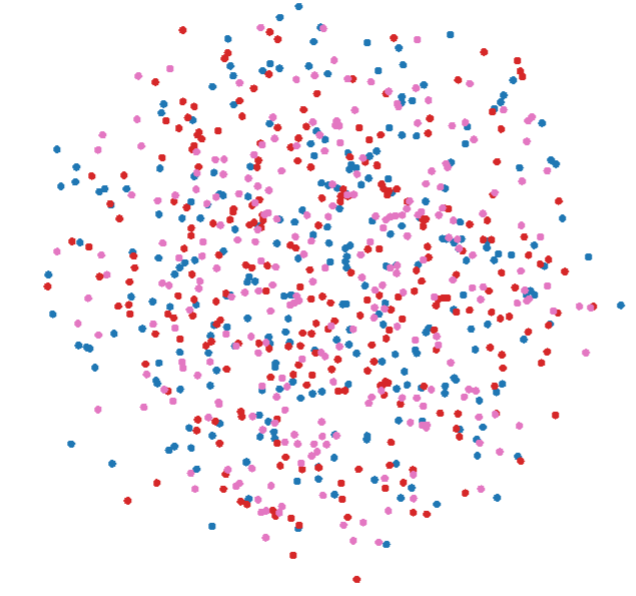
\includegraphics[width=\linewidth]{chapters/prime/figs/latent.png}
%     \vspace{-0.1in}
% \end{wrapfigure}
% objective-conditioned GAN model to 0.5 discriminator accuracy on our offline dataset, and often observed a collapse of the discriminator.
% %
% As a result, we trained a $\delta-$VAE~\citep{razavi2019preventing}, conditioned on the objective function (i.e., latency).
% %
% A standard VAE~\citep{kingma2013auto} suffered from posterior collapse and thus informed our choice of utilizing a $\delta-$VAE. 
% %
% The latent space of a trained objective-conditioned $\delta-$VAE corresponding to accelerators on a held-out validation dataset (not used for training) is visualized in the t-SNE plot in the figure on the right.
% %
% This is a 2D t-SNE of the accelerators configurations (\S Table~\ref{tab:arch_params}). 
% %
% The color of a point denotes the latency value of the corresponding accelerator configuration, partitioned into three bins. 
% %
% Observe that while we would expect these objective conditioned models to disentangle accelerators with different objective values in the latent space, the models we trained did not exhibit such a structure, which will hamper optimization.
% %
% While our method \primemethodname\ could also benefit from a generative optimizer (i.e., by using a generative optimizer in place of $\mathrm{Opt}(\cdot)$ with a conservative surrogate), we leave it for future work to design effective generative optimizers on the accelerator manifold.


\paragraph{Comparison to P3BO.}
%
We perform a comparison against P3BO, a state-of-the-art online method in biological sequence design~\citep{p3bo:arxiv:2020}.
%
On average, \primemethodname\ outperforms the P3BO method by 2.5$\times$ (up to 8.7$\times$ in U-Net).
%
In addition, we present the comparison between the total simulation runtime of the P3BO and Evolutionary methods in Figure~\ref{fig:converg_p3bo_evolutionary}.
%
Note that, not only the total simulation time of P3BO is around 3.1$\times$ higher than the Evolutionary method, but also the latency of final optimized accelerator is around 18\% for MobileNetEdgeTPU.
%
On the other hand, the total simulation time of \primemethodname\ for the task of accelerator design for MobileNetEdgeTPU is lower than both methods (only 7\% of the Evolutionary method as shown in Figure~\ref{fig:convergence_time}).
%
\begin{table}[H]
\small
\centering
\vspace*{0.1cm}
\caption{Optimized objective values (i.e., latency in milliseconds) obtained by \primemethodname\ and P3BO~\citep{p3bo:arxiv:2020} when optimizing over single applications (MobileNetEdgeTPU, \mfour, t-RNN Dec, t-RNN Enc, and U-Net). On average, \primemethodname\ outperforms P3BO by 2.5$\times$.}
\label{table:p3bo_vs_prime}
\resizebox{0.7\textwidth}{!}{
\begin{tabular}{l||l||l}
\toprule
\textbf{Application}&\textbf{\primemethodname~}\textbf{(Ours)}&\textbf{P3BO}\\\midrule
MobileNetEdgeTPU&\textbf{298.50}&376.02\\\hline
\mfour&\textbf{370.45}&483.39\\\hline
U-Net&\textbf{740.27}&771.70\\\hline
t-RNN Dec&\textbf{132.88}&865.12\\\hline
t-RNN Enc&\textbf{130.67}&1139.48\\\bottomrule
\CC \textbf{Geomean of \primemethodname's Improvement}&\CC~\texttt{\textbf{1.0$\times$}}&\CC~\texttt{\textbf{2.5$\times$}}\\
\bottomrule
\end{tabular}
}
\vspace{-0.1cm}
\end{table}
%
\begin{figure}[t!]
    \centering
    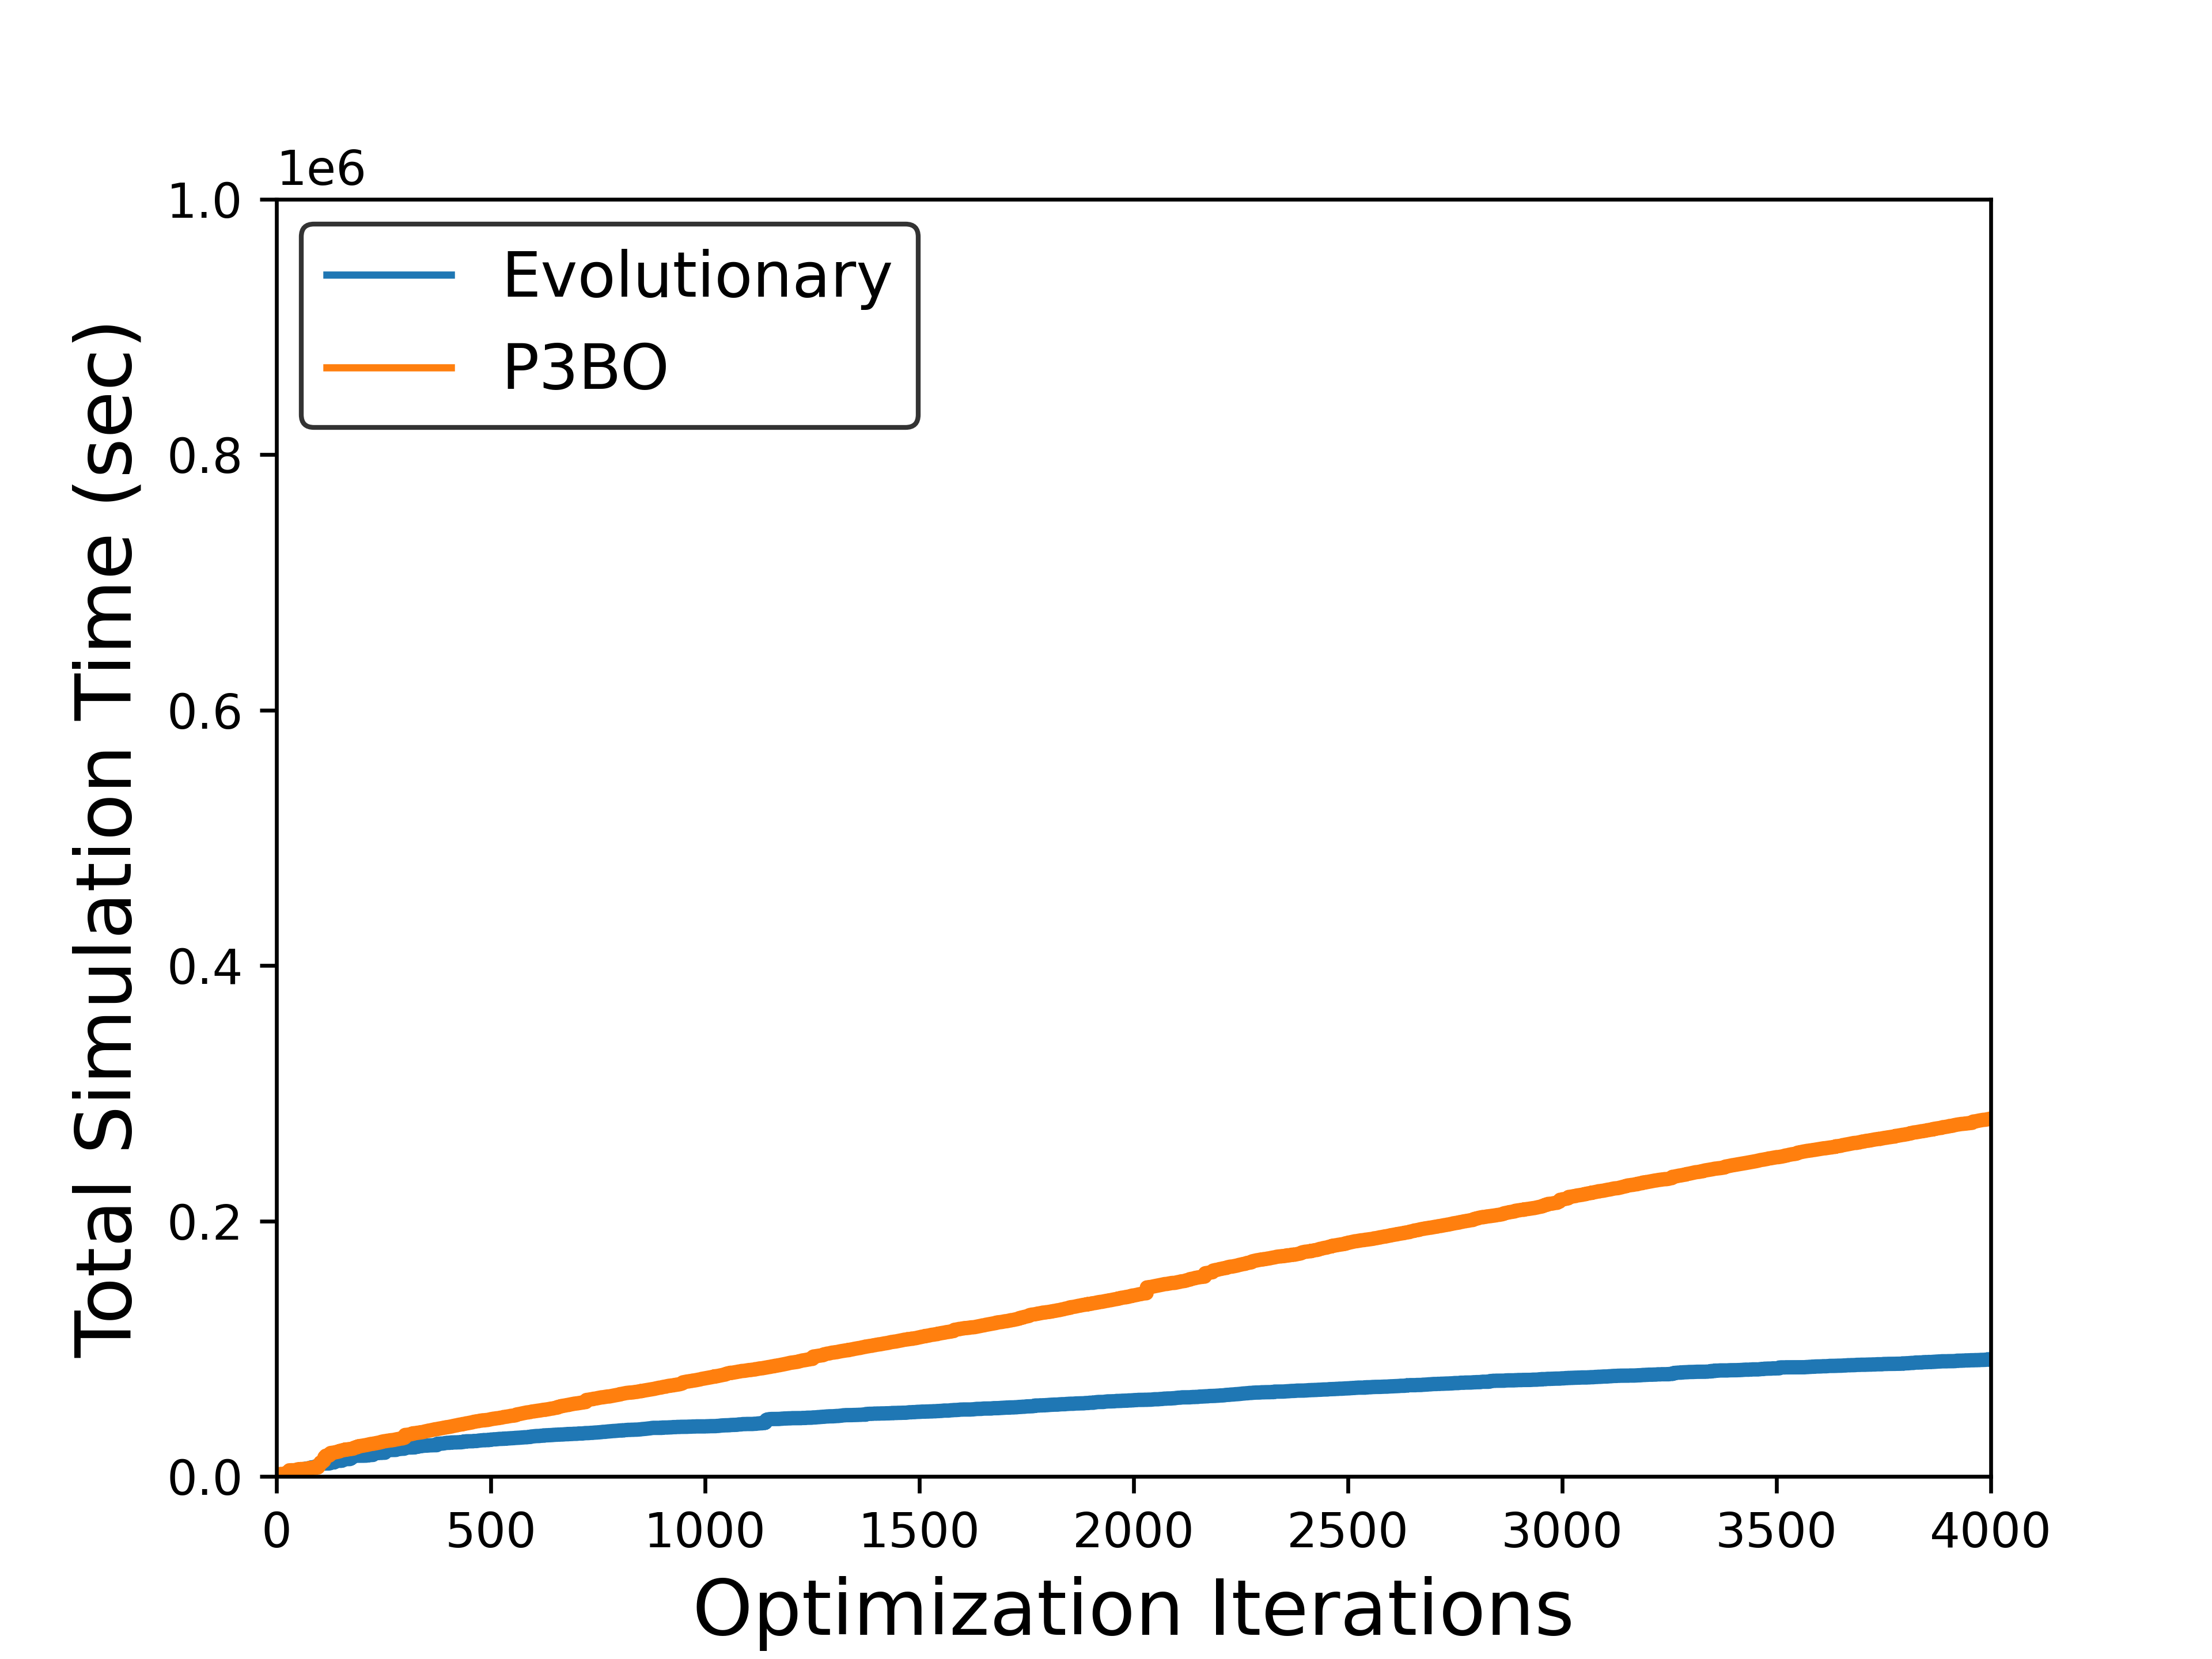
\includegraphics[width=0.5\textwidth]{chapters/prime/figs/convergence_time_v2_evolutionary_vs_p3bo.png}
    \caption{Comparing the total simulation time needed by the P3BO and Evolutionary method on MobileNetEdgeTPU. Note that, not only the total simulation time of P3BO is around 3.1$\times$ higher than the Evolutionary method, but also the latency of final optimized accelerator is around 18\% for MobileNetEdgeTPU. The total simulation time of our method is around 7\% of the Evolutionary method (See Figure~\ref{fig:convergence_time}).}
    \label{fig:converg_p3bo_evolutionary}
    \vspace{-0.1in}
\end{figure}
%

%



\subsection{Learned Surrogate Model Reuse for Accelerator Design}
\label{app:additional_experiments_multi}
%
Extending our results in Table~\ref{table:results_multi_task}, we present another variant of optimizing accelerators jointly for multiple applications. In that scenario, the learned conservative model is reused to architect an accelerator for a subset of applications used for training. We train a contextual conservative model on the variants of MobileNet (Table~\ref{tab:models}) as discussed in Section~\ref{sec:method}, but generated optimized designs by only optimizing the average surrogate on only two variants of MobileNet (MobileNetEdgeTPU and MobileNetV2). This tests the ability of our approach \primemethodname\ to provide a general contextual conservative surrogates, that can be trained \textit{only once} and optimized multiple times with respect to different subsets of applications. Observe in Table~\ref{table:results_edge_v2}, \primemethodname\ architects high-performing accelerator configurations (better than the best point in the dataset by 3.29$\times$ -- last column) while outperforming the online optimization methods by 7\%.
%
\begin{table}[t!]
\small
\renewcommand{\arraystretch}{1.2}
\centering
\caption{Optimized objective values (i.e., latency in milliseconds) obtained by our \primemethodname\ when using the jointly optimized model on three variants of MobileNets and use for MobileNetEdgeTPU and MobileNetV2 for different dataset configurations. \primemethodname\ outperforms the best online method by \textbf{7\%} and finds an accelerator that is \textbf{3.29$\times$} better than the best accelerator in the training dataset (last row). The best accelerator configuration is highlighted in bold.}
\label{table:results_edge_v2}
\resizebox{\textwidth}{!}{
\begin{tabular}{l||l||l|l||l|l|l||l}
\toprule
&\multicolumn{3}{c||}{\textbf{\primemethodname}}& &\multicolumn{2}{c||}{\textbf{Online Optimization}}&\\\cline{2-4}\cline{6-7}
\textbf{Applications}&\textbf{All}& \textbf{-Opt}&\textbf{-Infeasible}&\textbf{Standard}& \textbf{Bayes Opt}&\textbf{Evolutionary}&\textbf{$\mathcal{D}$ (Best in Training)}\\\midrule
(MobileNetEdgeTPU, MobileNetV2)&\textbf{253.85}&297.36&264.85&341.12&275.21&271.71&834.68\\
\bottomrule
\end{tabular}
}
\end{table}


%
\subsection{Learned Surrogate Model Reuse under Different Design Constraint}
\label{app:transfer}

\begin{table}[t!]
    \small
    \renewcommand{\arraystretch}{1.2}
    \centering
    \caption{Optimized objective values (i.e., latency in milliseconds) obtained by various methods for the task of learning accelerators specialized to MobileNetEdgeTPU under chip area budget constraint 18~mm$^2$ reusing the already learned model by our method for MobileNetEdgeTPU (shown in Table~\ref{table:results_single_task}). Lower latency/runtime is better. From left to right: our method, our method without negative sampling (``\primemethodname-$\mathrm{Opt}$'') and without utilizing infeasible points (``\primemethodname-Infeasible''), standard surrogate (``Standard''), online Bayesian optimization (``Bayes Opt''), online evolutionary algorithm (``Evolutionary'') and the best design in the training dataset. Note that \primemethodname\ improves over the best in the dataset by 12\%, outperforms the best online optimization method by 4.4\%. The best accelerator configuration is highlighted in bold.}
    \label{table:results_edge_18}
    \resizebox{\textwidth}{!}{
    \begin{tabular}{l||l||l|l||l|l|l||l}
    \toprule
    &\multicolumn{3}{c||}{\textbf{\primemethodname}}& &\multicolumn{2}{c||}{\textbf{Online Optimization}}&\\\cline{2-4}\cline{6-7}
    \textbf{Applications}&\textbf{All}& \textbf{-Opt}&\textbf{-Infeasible}&\textbf{Standard}& \textbf{Bayes Opt}&\textbf{Evolutionary}&\textbf{$\mathcal{D}$ (Best in Training)}\\\midrule
    MobileNetEdgeTPU, Area $\leq$ 18~mm$^2$&\textbf{315.15}&433.81&351.22&470.09&331.05&329.13&354.13\\
    \bottomrule
    \end{tabular}
    }
    \end{table}
    %
%
We also test the robustness of our approach in handling variable constraints at test-time such as different chip area budget.
%
We evaluate the learned conservative surrogate trained via \primemethodname\ under a reduced value of the area threshold, $\alpha$, in Equation~\ref{eqn:opt_prob}.
%
To do so, we utilize a variant of rejection sampling -- we take the learned model trained for a default area constraint $\alpha = 29~\mathrm{mm}^2$ and then reject all optimized accelerator configurations which do not satisfy a reduces area constraint: $\mathrm{Area}(\rvx) \leq \alpha_0 = 18~\mathrm{mm}^2$.
%
Table~\ref{table:results_edge_18} summarizes the results for this scenario for the MobileNetEdgeTPU~\citep{edgetpu:arxiv:2020} application under the new area constraint ($\alpha = 18~\mathrm{mm}^2$).
%
A method that produces diverse designs which are both high-performing and are spread across diverse values of the area constraint are expected to perform better.
%
As shown in Table~\ref{table:results_edge_18}, \primemethodname\ provides better accelerator than the best online optimization from scratch with the new constraint value by 4.4\%, even when \primemethodname\ does not train its conservative surrogate with this unseen test-time design constraint.
%
Note that, when the design constraint changes, online methods generally need to restart the optimization process from scratch and undergo costly queries to the simulator.
%
This would impose additional overhead in terms of total simulation time (\S~Figure~\ref{fig:convergence_time} and Figure~\ref{fig:convergence_time_seven_models}). However, the results in Table~\ref{table:results_edge_18} shows that our learned surrogate model can be reused under different test-time design constraint eliminating additional queries to the simulator.
%



\subsection{Analysis of Designed Accelerators}
\label{app:analysis}
%
\begin{table}[t!]
\small
\renewcommand{\arraystretch}{1.2}
\centering
\caption{Per application latency for the best accelerator design suggested by \primemethodname\ and the Evolutionary method according to Table~\ref{table:results_multi_task} for multi-task accelerator design (nine applications and area constraint 100~mm$^2$). \primemethodname\ outperforms the Evolutionary method by 1.35$\times$.}
\label{table:per_application_latency}
\resizebox{0.9\textwidth}{!}{
\begin{tabular}{l|r|r|r}
\toprule
&\multicolumn{2}{c|}{\textbf{Latency (ms)}}&\\\cline{2-3}
\textbf{Applications}&\textbf{\primemethodname}&\textbf{Evolutionary~(Online)}&\textbf{Improvement of \primemethodname\ over Evolutionary}\\\midrule
{MobileNetEdgeTPU}&\textbf{288.38}&319.98&1.10$\times$\\\hline
{MobileNetV2}&\textbf{216.27}&255.95&1.18$\times$\\\hline
{MobileNetV3}&\textbf{487.46}&573.57&1.17$\times$\\\hline
{\mfour}&\textbf{400.88}&406.28&1.01$\times$\\\hline
{\mfive}&248.18&\textbf{239.18}&0.96$\times$\\\hline
{\msix}&164.98&\textbf{148.83}&0.90$\times$\\\hline
{U-Net}&1268.73&\textbf{908.86}&0.71$\times$\\\hline
{t-RNN Dec}&\textbf{191.83}&862.14&5.13$\times$\\\hline
{t-RNN Enc}&\textbf{185.41}&952.44&4.49$\times$\\\bottomrule
\CC \textbf{Average~(Latency in ms)}&\CC~\texttt{\textbf{383.57}}&\CC~\texttt{\textbf{518.58}}&\CC~\texttt{\textbf{1.35$\times$}}\\\bottomrule
\end{tabular}
}
\end{table}
\begin{table}[t!]
\small
\renewcommand{\arraystretch}{1.2}
\centering
\caption{Optimized accelerator configurations (See Table~\ref{tab:arch_params}) found by \primemethodname\ and the Evolutionary method for multi-task accelerator design (nine applications and area constraint 100~mm$^2$). Last row shows the accelerator area in mm$^2$. \primemethodname\ reduces the overall chip area usage by 1.97$\times$. The difference in the accelerator configurations are shaded in gray.}
\label{table:best_accelerator_config}
\resizebox{0.6\textwidth}{!}{
\begin{tabular}{l|r|r}
\toprule
&\multicolumn{2}{c}{\textbf{Parameter Value}}\\\cline{2-3}
\textbf{Accelerator Parameter}&\textbf{\primemethodname}&\textbf{Evolutionary~(Online)}\\\midrule
\# of PEs-X&4&4\\\hline
\CC{}\# of PEs-Y&\CC~6&\CC~8\\\hline
\CC{}\# of Cores&\CC~64&\CC~128\\\hline
\CC{}\# of Compute Lanes&\CC~4&\CC~6\\\hline
\CC{}PE Memory&\CC~2,097,152&\CC~1,048,576\\\hline
Core Memory&131,072&131,072\\\hline
\CC{}Instruction Memory&\CC~32,768&\CC~8,192\\\hline
Parameter Memory&4,096&4,096\\\hline
\CC{}Activation Memory&\CC~512&\CC~2,048\\\hline
DRAM Bandwidth~(Gbps)&30&30\\\bottomrule
\CC~\textbf{Chip Area~(mm$^2$)}&\CC~\texttt{\textbf{46.78}}&\CC~\texttt{\textbf{92.05}}\\\bottomrule
\end{tabular}
}
\end{table}
%
In this section, we overview the best accelerator configurations that \primemethodname\ and the Evolutionary method identified for multi-task accelerator design (See Table~\ref{table:results_multi_task}), when the number of target applications are nine and the area constraint is set to 100~mm$^2$.
%
The average latencies of the best accelerators found by \primemethodname\ and the Evolutionary method across nine target applications are \textbf{383.57~ms} and \textbf{518.58~ms}, respectively.
%
In this setting, our method outperforms the best online method by \textbf{1.35$\times$}.
%
Table~\ref{table:per_application_latency} shows per application latencies for the accelerator suggested by our method and the Evolutionary method.
%
The last column shows the latency improvement of \primemethodname\ over the Evolutionary method. Interestingly, while the latency of the accelerator found by our method for MobileNetEdgeTPU, MobileNetV2, MobileNetV3, \mfour, t-RNN Dec, and t-RNN Enc are better, the accelerator identified by the online method yields lower latency in \mfive, \msix, and U-Net.

%
To better understand the trade-off in design of each accelerator designed by our method and the Evolutionary method, we present all the accelerator parameters (See Table~\ref{tab:arch_params}) in Table~\ref{table:best_accelerator_config}.
%
The accelerator parameters that are different between each of the designed accelerator are shaded in gray (e.g. \# of PEs-Y, \# of Cores, \# of Compute Lanes, PE Memory, Instruction Memory, and Activation Memory).
%
Last row of Table~\ref{table:best_accelerator_config} depicts the overall chip area usage in mm$^2$. \primemethodname\ not only outperforms the Evolutionary algorithm in reducing the average latency across the set of target applications, but also reduces the overall chip area usage by \textbf{1.97$\times$}.
%
Studying the identified accelerator configuration, we observe that \primemethodname\ trade-offs compute (\colorbox{lightgray}{\textbf{64 cores vs. 128 cores}}) for larger PE memory size (\colorbox{lightgray}{\textbf{2,097,152 vs. 1,048,576}}). These results show that \primemethodname\ favors PE memory size to accommodate for the larger memory requirements in t-RNN Dec and t-RNN Enc (See Table~\ref{tab:models} Model Parameters) where large gains lie.
%
Favoring larger on-chip memory comes at the expense of lower compute power in the accelerator. This reduction in the accelerator's compute power leads to higher latency for the models with large number of compute operations, namely \mfive, \msix, and U-Net (See last row in Table~\ref{tab:models}).
%
\mfour is an interesting case where both compute power and on-chip memory is favored by the model (6.23~MB model parameters and 3,471,920,128 number of compute operations). This is the reason that the latency of this model on both accelerators, designed by our method and the Evolutionary method, are comparable (400.88~ms in \primemethodname\ vs. 406.28~ms in the online method).


\subsection{Comparison with Online Methods in Zero-Shot Setting}
\label{sec:app_zero_shot}
%
We evaluated the Evolutionary (online) method under two protocols for the last two rows of Table~\ref{table:zero_shot}: first, we picked the best designs (top-performing 256 designs similar to the \primemethodname\ setting in Section~\ref{sec:method}) found by the evolutionary algorithm on the training set of applications and evaluated them on the target applications and second, we let the evolutionary algorithm continue simulator-driven optimization on the target applications.
%
The latter is unfair, in that the online approach is allowed access to querying more designs in the simulator. Nevertheless, we found that in either configuration, the evolutionary approach performed worse than \primemethodname\, which does not access training data from the target application domain.
%
For the area constraint 29~mm$^2$ and 100~mm$^2$, the Evolutionary algorithm reduces the latency from 1127.64~$\rightarrow$~820.11 and 861.69~$\rightarrow$~552.64, respectively, although still worse than \primemethodname.
%
In the second experiment in which we \emph{unfairly} allow the evolutionary algorithm to continue optimizing on the target application, the Evolutionary algorithm suggests worse designs than Table~\ref{table:zero_shot} (e.g. 29~mm$^2$: 1127.64~$\rightarrow$~1181.66 and 100~mm$^2$: 861.69~$\rightarrow$~861.66).
%


\subsection{\primemethodname\ Ablation Study}
\label{sec:appx_ablation}



\begin{table}[t]
\vspace{5pt}
\centering
\caption{\label{table:appx_results_single_task}{Optimized objective values (i.e., latency in milliseconds) obtained by various methods for the task of learning accelerators specialized to a given application. Lower latency/runtime is better. From left to right: our method, our method without negative sampling (``\primemethodname-$\mathrm{Opt}$'') and without utilizing infeasible points (``\primemethodname-Infeasible''), standard surrogate (``Standard''), online Bayesian optimization (``Bayes Opt''), online evolutionary algorithm (``Evolutionary'') and the best design in the training dataset. Note that, in all the applications \primemethodname\ improves over the best in the dataset, outperforms online optimization methods in 7/9 applications and the complete version of \primemethodname\ generally performs best. The best accelerator designs are in bold.}}
% \renewcommand{\arraystretch}{1.2}
\resizebox{1.0\textwidth}{!}{\begin{tabular}{l||r|r|r||r||r|r||r}
\hline
&\multicolumn{3}{c||}{\textbf{\primemethodname}}&&\multicolumn{2}{c||}{\textbf{Online Optimization}}&\\\cline{2-4}\cline{6-7}
\textbf{Application}&\textbf{All}& \textbf{-Opt}&\textbf{-Infeasible}&\textbf{Standard}&\textbf{Bayes Opt}&\textbf{Evolutionary}&\textbf{$\mathcal{D}$ (Best in Training)}\\\midrule
MobileNetEdge&\textbf{298.50}&435.40&322.20&411.12&319.00&320.28&354.13\\\hline
MobileNetV2&\textbf{207.43}&281.01&214.71&374.52&240.56&238.58&410.83\\\hline
MobileNetV3&\textbf{454.30}&489.45&483.96&575.75&534.15&501.27&938.41\\\hline
\mfour&\textbf{370.45}&478.32&432.78&1139.76&396.36&383.58&779.98\\\hline
\mfive&208.21&319.61&246.80&307.57&201.59&\textbf{198.86}&449.38\\\hline
\msix&131.46&197.70&162.12&180.24&121.83&\textbf{120.49}&369.85\\\hline
U-Net&\textbf{740.27}&740.27&765.59&763.10&872.23&791.64&1333.18\\\hline
t-RNN Dec&\textbf{132.88}&172.06&135.47&136.20&771.11&770.93&890.22\\\hline
t-RNN Enc&\textbf{130.67}&134.84&137.28&150.21&865.07&865.07&584.70\\\bottomrule
\end{tabular}}
\normalsize
% \vspace{-16pt}
\end{table}

Here we ablate over variants of our method: (1) $\mathrm{Opt}$ was not used for negative sampling (``\primemethodname-$\mathrm{Opt}$'' in Table~\ref{table:appx_results_single_task}) (2)  infeasible points were not used (``\primemethodname-Infeasible'' in Table~\ref{table:appx_results_single_task}).
%
As shown in Table~\ref{table:appx_results_single_task}, the variants of our method generally performs worse compared to the case when both negative sampling and infeasible data points are utilized in training the surrogate model.

\subsection{{Comparison with Human-Engineered Accelerators}}
\label{app:human_engineered}
%
{In this section, we compare the optimized accelerator design found by \primemethodname\ that is targeted towards single applications to the manually optimized EdgeTPU design~\citep{yazdanbakhsh2021evaluation,edgetpu:arxiv:2020}.
%
EdgeTPU accelerators are primarily optimized towards running applications in image classification, particularly, MobileNetV2,  MobileNetV3 and MobileNetEdgeTPU.
%
The goal of this comparison is to present the potential benefit of \primemethodname for a dedicated application when compared to human designs.
%
For this comparison, we utilize an area constraint of 27~mm$^2$ and a DRAM bandwidth of 25 Gbps, to match the specifications of the EdgeTPU accelerator.}
%

{Table~\ref{table:edgetpu_comparison} shows the summary of results in two sections, namely ``Latency'' and ``Chip Area''. The first and second under each section show the results for \primemethodname\ and EdgeTPU, respectively.
%
The final column for each section shows the improvement of the design suggested by \primemethodname\ over EdgeTPU.
%
On average (as shown in the last row), \primemethodname\ finds accelerator designs that are 2.69$\times$ (up to 11.84$\times$ in t-RNN Enc) better than EdgeTPU in terms of latency. Our method achieves this improvement while, on average, reducing the chip area usage by 1.50$\times$ (up to 2.28$\times$ in MobileNetV3). Even on the MobileNet image-classification domains, we attain an average improvement of 1.85$\times$.}

\begin{table}[t!]
\small
\vspace{0.1in}
\renewcommand{\arraystretch}{1.2}
\centering
\caption{\review{The comparison between the accelerator designs suggested by \primemethodname\ and EdgeTPU~\citep{yazdanbakhsh2021evaluation,edgetpu:arxiv:2020} for single model specialization. On average (last row), with single-model specialization our method reduces the latency by 2.69$\times$ while minimizes the chip area usage by 1.50$\times$.}}
\label{table:edgetpu_comparison}
\resizebox{\textwidth}{!}{
\begin{tabular}{l|r|r|r||r|r|r}
\toprule
&\multicolumn{3}{c||}{\textbf{Latency~(milliseconds)}}&\multicolumn{3}{c}{\textbf{Chip Area~(mm$^2$)}}\\\cline{2-7}
\textbf{Application}&\textbf{\primemethodname}&\textbf{EdgeTPU}&\textbf{Improvement}&\textbf{\primemethodname}&\textbf{EdgeTPU}&\textbf{Improvement}\\\midrule
MobileNetEdgeTPU&294.34&523.48&1.78$\times$&18.03&27&1.50$\times$\\\hline
MobileNetV2&208.72&408.24&1.96$\times$&17.11&27&1.58$\times$\\\hline
MobileNetV3&459.59&831.80&1.81$\times$&11.86&27&2.28$\times$\\\hline
\mfour&370.45&675.53&1.82$\times$&19.12&27&1.41$\times$\\\hline
\mfive&208.42&377.32&1.81$\times$&22.84&27&1.18$\times$\\\hline
\msix&132.98&234.88&1.77$\times$&16.93&27&1.59$\times$\\\hline
U-Net&1465.70&2409.73&1.64$\times$&25.27&27&1.07$\times$\\\hline
t-RNN Dec&132.43&1384.44&10.45$\times$&14.82&27&1.82$\times$\\\hline
t-RNN Enc&130.45&1545.07&11.84$\times$&19.87&27&1.36$\times$\\\bottomrule
\CC~\textbf{Average Improvement}&\CC~---&\CC~---&\CC~\textbf{2.69$\times$}&\CC~---&\CC~---&\CC~\textbf{1.50$\times$}\\\bottomrule
\end{tabular}
}
\end{table}
%



\subsection{{Zero-Shot Results on All Applications}}
\review{In this section, we present the results of zero-shot optimization from Table~\ref{table:zero_shot} on all the nine applications we study in the paper (i.e., test applications = all nine models: MobileNet (EdgeTPU, V2, V3), \msix, \mfive, \mfour, t-RNN (Enc and Dec), and U-Net). We investigate this for two sets of training applications and two different area budgets. As shown in Table~\ref{table:zero_shot_all}, we find that \primemethodname\ does perform well compared to the online evolutionary method.}

\begin{table*}[t]
\small
\centering
\vspace*{0.0cm}
\caption{\label{table:zero_shot_all}\review{Optimized objective values (i.e., latency in milliseconds) under zero-shot setting when the test applications include all the nine evaluated models (e.g. MobileNet (EdgeTPU, V2, V3), \mfour, \mfive, \msix, t-RNN Dec, t-RNN Enc, U-Net). Lower latency is better. From \textbf{left} to \textbf{right}: the applications used to train the surrogate model in \primemethodname\, the target applications for which the accelerator is optimized for, the area constraint of the accelerator, \primemethodname's (best, median) latency, and best online method's (best, median) latency. The best accelerator configurations identified is highlighted in bold.}}
\vspace{-0.1cm}
\resizebox{\textwidth}{!}{% <------ Don't forget this %
\begin{tabular}{l|l|l|l}
\toprule
\textbf{Train Applications}&\textbf{Area}&\textbf{\primemethodname}&\textbf{Evolutionary~(Online)}\\\midrule
% Train = MobilenetEdge, MobilenetV3, Target = MobilenetV2
% MobileNet~(Edge, V3)&{MobileNetV2}&29~mm$^2$&(\textbf{311.39}, \textbf{313.76})&(314.31, 316.65)\\\hline
% MobileNet~(V2, V3), \mfive, \msix&{MobileNetEdge, \mfour}&29~mm$^2$&(357.05, 364.92)&(\textbf{354.59}, \textbf{357.29})\\\hline
% Area 29
MobileNet~(EdgeTPU,V2,V3), \mfour, \mfive, \msix, t-RNN Enc&29~mm$^2$&(\textbf{426.65}, \textbf{427.94})&(586.55, 586.55)\\\hline
% Area 100
MobileNet~(EdgeTPU,V2,V3), \mfour, \mfive, \msix, t-RNN Enc&100~mm$^2$&(\textbf{365.95}, \textbf{366.64})&(518.58, 519.37)\\\bottomrule
\CC \textbf{Geomean of \primemethodname's Improvement}&\CC--- &\CC~(1.0$\times$, 1.0$\times$)&\CC~(\texttt{\textbf{1.40$\times$}}, \texttt{\textbf{1.39$\times$}})\\
\bottomrule
\end{tabular}% <------ Don't forget this %
}
% \vspace{-0.2cm}
\end{table*}


\subsection{{Different Train and Validation Splits}}
{In the main paper, we used the worst 80\% of the feasible points in the training dataset for training and used the remaining 20\% of the points for cross-validation using our strategy based on Kendall's rank correlation. In this section, we explore some alternative training-validation split strategies to see how they impact the results. To do so, we consider two alternative strategies: \textbf{(1)} training on 95\% of the worst designs, validation on top 5\% of the designs, and \textbf{(2)} training on the top 80\% of the designs and validation on the worst 20\% of the designs. We apply these strategies to MobileNetEdgeTPU, \msix and t-RNN Enc models from Table~\ref{table:results_single_task}, and present a comparative evaluation in Table~\ref{table:train_val_split} below.}

{\textbf{Results.} As shown in Table~\ref{table:train_val_split}, we find that cross-validating using the best 5\% of the points in the dataset led to a reduced latency (298.50 $\rightarrow$ 273.30) on MobileNetEdgeTPU, and retained the same performance on \msix. However, it increased the latency on t-RNN Enc (130.67 $\rightarrow$ 137.45). This indicates at the possibility that while top 5\% of the datapoints can provide a better signal for cross-validation in some cases, this might also hurt performance if the size of the 5\% dataset becomes extremely small (as in the case of t-RNN Enc, the total dataset size is much smaller than either MobileNetEdgeTPU or \msix).}

{The strategy of cross-validating using the worst 20\% of the points hurt performance on \msix and t-RNN Enc, which is perhaps as expected, since the worst 20\% of the points may not be indicative of the best points found during optimization. However, while it improves performance on the MobileNetEdgeTPU application compared to the split used in the main paper but it is still worse than using the top 5\% of the points for validation.}
%
\begin{table}[H]
\small
\centering
% \vspace*{0.1cm}
\caption{\review{Performance of \primemethodname\ (as measured by median latency of the accelerator found across five runs) under various train-test splits on three applications studied in Table~\ref{table:results_single_task}.}}
\label{table:train_val_split}
\resizebox{0.99\textwidth}{!}{
\begin{tabular}{l|c|c|c}
\toprule
\textbf{Applications}&\textbf{Best 5\% Validation}&\textbf{Best 20\% Validation (Table~\ref{table:results_single_task})}&\textbf{Worst 20\% Validation}\\\midrule
MobileNetEdgeTPU&273.30&298.50&286.53\\\hline
\msix&131.46&131.46&142.68\\\hline
t-RNN Enc&137.45&130.67&135.71\\\bottomrule
\end{tabular}
}
\vspace{-0.1cm}
\end{table}
%


\section{Details of \primemethodname}
\label{app:details}
%
In this section, we provide training details of our method \primemethodname\ including hyperparameters and compute requirements and details of different tasks. 
%
\subsection{Hyperparameter and Training Details}
\label{sec:practical_implementation}
%
Algorithm~\ref{alg:prime} outlines our overall system for accelerator design.
%
\primemethodname\ parameterizes the function $f_\theta(\rvx)$ as a deep neural network as shown in Figure~\ref{fig:method}. 
%
The architecture of $f_\theta(\rvx)$ first embeds the discrete-valued accelerator configuration $\rvx$ into a continuous-valued 640-dimensional embedding via two layers of a self-attention transformer~\citep{vaswani2017attention}. 
%
Rather than directly converting this 640-dimensional embedding into a scalar output via a simple feed-forward network, which we found a bit unstable to train with Equation~\ref{eqn:final_training}, possibly due to the presence of competing objectives for a comparison), we pass the 640-dimensional embedding into $M$ different networks that map it to $M$ different scalar predictions $(f^i_\theta(\rvx))_{i=1}^M$. 
%
Finally, akin to attention~\citep{vaswani2017attention} and mixture of experts~\citep{shazeer2017outrageously}, we train an additional head to predict weights $(w_i)_{i=1}^M \geq 0$ of a linear combination of the predictions at different heads that would be equal to the final prediction: $f_\theta(\rvx) = \sum_{i=1}^K w_i f^i_\theta(\rvx)$.
%
Such an architecture allows the model to use different predictions $f^i_\theta(\rvx)$, depending upon the input, which allows for more stable training. To train $f_\theta(\rvx)$, we utilize the Adam~\citep{kingma2014adam} optimizer.
%
Equation~\ref{eqn:final_training} utilizes a procedure $\mathrm{Opt}$ that maximizes the learned function approximately. We utilize the same technique as Section~\ref{sec:method} (``optimizing the learned surrogate'') to obtain these negative samples.
%
We periodically refresh $\mathrm{Opt}$, once in every 20K gradient steps on $f_\theta(\rvx)$ over training.
\begin{algorithm}[ht] %b
  \caption{Training the conservative surrogate in PRIME}\label{alg:prime}
  \begin{algorithmic}[1]
    \State Initialize a neural model $f_{\theta_0}(\rvx)$ and a set $M = 23$ of negative particles to be updated by the firefly optimizer $\{\rvx^{-}_1(0), \cdots,  \rvx^{-}_i(0), \rvx^{-}_M(0)\}$ to random configurations from the design space.
    \For{iteration $i = 0, 1, 2, 3, \dots $ until convergence}
        \For{firefly update step  $t = 0, 1, \dots,  4$  \hfill \Comment{\textbf{Inner loop}}}
          \State Update the $M$ fireflies according to the firefly update rule in Equation~\ref{eqn:firefly1},\\ ~~~~~~~~~~~~towards maximizing $f_{\theta_i}(\rvx)$ according to: \hfill \Comment{\textbf{Negative mining}}\\ ~~~~~~~~~~~~~~~~~~~~~~~~~~~~~~~~${\rvx_{i}(ti+ 1) = \rvx_{i}(ti) + \beta(\rvx_{i}(ti) - \rvx_{j}(ti)) + {\eta}\epsilon_{ti}}$
      \EndFor
      \State Find the best firefly found in these steps to be used as the negative sample:\\ ~~~~~~~~~~~~~~~~~~~~~~$\rvx^{-}_i = \arg \min \{f_{\theta_i}(\rvx^{-}_1(t i)), \cdots, f_{\theta_i}(\rvx^{-}_M(t i))\}$ \hfill \Comment{\textbf{Find negative sample}}
      \State Run one gradient step on $\theta_i$ using Equation~\ref{eqn:final_training} with $\rvx^{-}_i$ as the negative sample
      \State \textbf{if} $i \% p == 0$, (p = 20000), then: \hfill \Comment{\textbf{Periodically reinitialize the optimizer}} \\~~~~~~~~~~~~~~~Reinitialize firefly particles  $\{\rvx^{-}_1(0), \cdots,  \rvx^{-}_i(0), \rvx^{-}_M(0)\}$ to random designs.
    \EndFor
    \State Return the final model $f_{\theta^*}(\rvx)$
  \end{algorithmic}
\end{algorithm}

The hyperparameters for training the conservative surrogate in Equations~\ref{eqn:final_training} and its contextual version are as follows:
\begin{itemize}
    \item \textbf{Architecture of ${f}_\theta(\rvx)$}. As indicated in Figure~\ref{fig:method}, our architecture takes in list of categorical (one-hot) values of different accelerator parameters (listed in Table~\ref{tab:arch_params}), converts each parameter into $64$-dimensional embedding, thus obtaining a $10 \times 64$ sized matrix for each accelerator, and then runs two layers of self-attention~\citep{vaswani2017attention} on it. The resulting $10 \times 64$ output is flattened to a vector in $\mathbb{R}^{640}$ and fed into $M = 7$ different prediction networks that give rise to $f^1_\theta(\rvx), \cdots, f^M_\theta(\rvx)$, and an additional attention 2-layer feed-forward network (layer sizes $=[256, 256]$) that determines weights $w_1, \cdots, w_M$, such that $w_i \geq 0$ and $\sum_{i=1}^M w_i = 1$. Finally the output is simply $f_\theta(\rvx) = \sum_i w_i f^i_\theta(\rvx)$. 
    \item \textbf{Optimizer/learning rate for training $f_\theta(\rvx)$}. Adam, $1e-4$, default $\beta_1 = 0.9$, $\beta_2 = 0.999$.
    \item \textbf{Validation set split.} Top 20\% high scoring points in the training dataset are used to provide a validation set for deciding coefficients $\alpha$, $\beta$ and the checkpoint to evaluate.
    \item \textbf{Ranges of $\alpha$, $\beta$.} We trained several $f_\theta(\rvx)$ models with $\alpha \in [0.0, 0.01, 0.1, 0.5, 1.0, 5.0]$ and $\beta \in [0.0, 0.01, 5.0, 0.1, 1.0]$. Then we selected the best values of $\alpha$ and $\beta$ based on the highest Kendall's ranking correlation on the validation set. Kendall's ranking correlation between two sets of objective values: $S = \{y_1, y_2, \cdots, y_N\}$ corresponding to ground truth latency values on the validation set and $S' = \{y'_1, y'_2, \cdots, y'_N \}$ corresponding to the predicted latency values on the validation set is given by $\tau$ equal to:
    \begin{equation}
        \tau = \frac{\sum_{i, j}^{N, N} \mathbb{I}[(y_i - y_j) (y'_i - y'_j) > 0] - \sum_{i, j}^{N, N} \mathbb{I}[(y_i - y_j) (y'_i - y'_j) \leq 0]}{N \cdot (N - 1)}.   
    \end{equation}
    \item \textbf{Clipping $f_\theta(\rvx)$ during training}. Equation~\ref{eqn:final_training} increases the value of the learned function $f_\theta(\rvx)$ at $\rvx = \rvx_0 \in \mathcal{D}_\text{infeasible}$ and $\rvx^- \sim \mathrm{Opt}(f_\theta)$. We found that with the small dataset, these linear objectives can run into numerical instability, and produce $+\infty$ predictions. To avoid this, we clip the predicted function value both above and below by $\pm 10000.0$, where the valid range of ground-truth values is $\mathcal{O}(1000)$.
    \item \textbf{Negative sampling with $\mathrm{Opt}(\cdot)$}. As discussed in Section~\ref{sec:method}, we utilize the firefly optimizer for both the negative sampling step and the final optimization of the learned conservative surrogate. When used during negative sampling, we refresh (i.e., reinitialize) the firefly parameters after every $p = 20000$ gradient steps of training the conservative surrogate, and run $t = 5$ steps of firefly optimization per gradient step taken on the conservative surrogate. 
    \item \textbf{Details of firefly:} The initial population of fireflies depends on the number of accelerator configurations ($\mathcal{C}$) following the formula $10+\round{(\mathcal{C}^{1.2}+\mathcal{C})\times0.5}$. In our setting with ten accelerator parameters (See Table~\ref{tab:arch_params}), the initial population of fireflies is 23. We use the same hyperparameters: $\gamma = 1.0, \beta_0 = 1.0$, for the optimizer in all the experiments and never modify it. The update to a particular optimization particle (i.e., a firefly) $\rvx_i$, at the $t$-th step of optimization is given by: 
    \begin{equation}
    \label{eqn:firefly1}
    \begin{aligned}
    {\rvx_{i}(t+1) = \rvx_{i}(t) + \beta(\rvx_{i}(t) - \rvx_{j}(t)) + ~\text{i.i.d. Gaussian noise},}
    \end{aligned}
    \end{equation}
    where $\rvx_j(t), j \neq i$ is a different firefly that achieves a better objective value compared to $\rvx_i$ and the function $\beta$ is given by: $\beta(r) = \beta_{0}e^{-\gamma{}r^2}$.
    \item \review{\textbf{Training set details:} The training dataset sizes for the studied applications are shown in Table~\ref{table:dataset_size}. To recap, to generate the dataset, we first randomly sampled accelerators from the deign space, and evaluated them for the target application, and constituted the training set from the worst-performing feasible accelerators for the given application. Since different applications admit different feasibility criteria (differences in compilation, hardware realization, and etc.), the dataset sizes for each application are different, as the number of feasible points is different. Note however that as mentioned in the main text, these datasets all contain $\leq 8000$ feasible points.}
    
    \review{\textbf{Discussion on data quality:} In the cases of t-RNN Dec, t-RNN Enc, and U-Net, we find that the number of feasible points is much smaller compared to other applications, and we suspect this is because our random sampling procedure does not find enough feasible points. This is a limitation of our data collection strategy and we intentionally chose this na\"ive strategy to keep data collection simple. Other techniques for improving data collection and making sure that the data does not consist of only infeasible points includes strategies such as utilizing logged data from past runs of online evolutionary methods, mixed with some data collected via random sampling to improve coverage of the design space.} 
\end{itemize}

\begin{table}[t]
    \small
    \centering
    \vspace*{0.1cm}
    \caption{\review{Dataset sizes for various applications that we study in this paper. Observe that all of the datasets are smaller than $8000$.}}
    \label{table:dataset_size}
    \resizebox{0.5\textwidth}{!}{
    \begin{tabular}{l||r}
    \toprule
    \textbf{Application}& \textbf{Dataset size}\\\midrule
    MobileNetEdgeTPU & 7697 \\\hline
    MobileNetV2 & 7620 \\ \hline
    MobileNetV3 & 5687 \\ \hline
    \mfour & 3763 \\ \hline
    \mfive & 5735 \\ \hline
    \msix & 7529 \\ \hline
    U-Net & 557\\\hline
    t-RNN Dec & 1211\\\hline
    t-RNN Enc & 1240\\\bottomrule
    \end{tabular}
    }
    \vspace{-0.1cm}
\end{table}

\subsubsection{\review{Details of Firefly Used for Our Online Evolutionary Method}}
\label{app:online_opt_details}

\review{In this section, we discuss some details for firefly optimization used in the online evolutionary method.}

{\textbf{Stopping criterion:} We stopped the firefly optimization when the latency of the best design found did not improve over the previous 1000 iterations, but we also made sure to run firefly optimization for at least 8000 iterations, to make sure that both the online and offline methods match in terms of the data budget. We also provide the convergence curves for firefly optimization on various single-application problems from Table~\ref{table:results_single_task} in Figure~\ref{fig:convergence_curves}.}

{\textbf{What happens if we run firefly optimization for longer?} We also experimented with running the evolutionary methods for longer (i.e., 32k simulator accesses compared to 8k), to check if this improves the performance of the evolutionary approach. As shown in Table~\ref{table:online_budget}, we find that while this procedure does improve performance in some cases, the performance does not improve much beyond 8k steps. This indicates that there is a possibility that online methods can perform better than \primemethodname\ if they are run for many more optimization iterations against the simulator, but they may not be as data-efficient as \primemethodname.}

\begin{table*}[t!]
\small
\centering
\vspace*{0.0cm}
\caption{\label{table:online_budget}\review{Comparing the latency of the accelerators designed by the evolutionary approach for variable number of simulator access budgets (8k and 32k). Even with $4\times$ as much allowed simulator interaction, online methods are unable to perform that well in our case.}}
\resizebox{0.95\textwidth}{!}{% <------ Don't forget this %
\begin{tabular}{l|l|l|l|l}
\toprule
&&&\multicolumn{2}{c}{\textbf{Evolutionary~(Online)}}\\\cline{4-5}
\textbf{Application}&\textbf{Area}&\textbf{\primemethodname}&\textbf{8k data points}&\textbf{32k data points}\\\midrule
MobileNetEdgeTPU&29~mm$^2$&298.50&320.28&311.35\\\hline
t-RNN Dec&29~mm$^2$&132.88&770.93&770.63\\\hline
t-RNN Enc&29~mm$^2$&130.67&865.07&865.07\\\bottomrule
\CC \textbf{Geomean of \primemethodname's Improvement}&\CC---&\CC~(1.0$\times$, 1.0$\times$)&\CC~\texttt{\textbf{3.45$\times$}}&\CC~\texttt{\textbf{3.42$\times$}}\\
\bottomrule
\end{tabular}% <------ Don't forget this %
}
\vspace{-0.3cm}
\end{table*}
%

{\textbf{Hyperparameter tuning for firefly:} Since the online optimization algorithms we run have access to querying the simulator over the course of training, we can simply utilize the value of the latest proposed design as a way to perform early stopping and hyperparameter tuning. A na\"ive way to perform hyperparameter tuning for such evolutionary methods is to run the algorithm for multiple rounds with multiple hyperparameters, however this is compute and time intensive. Therefore, we adopted a dynamic hyperparameter tuning strategy. Our implementation of the firefly optimizer tunes hyperparameters by scoring a set of hyperparameters based on its best performance over a sliding window of $T$ data points. This allows us to adapt to the best hyperparameters on the fly, within the course of optimization, effectively balancing the number of runs that need to be run in the simulator and hyperparameter tuning.}
\review{This dynamic hyperparameter tuning strategy requires some initial coverage of the hyperparameter space before hyperparameter tuning begins, and therefore, this tuning begins only after $750$ datapoints. 
After this initial phase, every $T = 50$ iterations, the parameters $\gamma$ and $\beta_0$ are updated via an evolutionary scoring strategy towards their best value.}

{\textbf{Discussion of t-RNN Enc and t-RNN Dec}. Finally, we discuss the results of the evolutionary approach on the t-RNN Enc and t-RNN Dec tasks, for which the convergence plots are shown in Figures~\ref{fig:conv_rnn_dec} and \ref{fig:conv_enc}. Observe that the best solution found by this optimization procedure converges quite quickly in this case (with about 1000 iterations) and the evolutionary method, despite the dynamic hyperparameter tuning is unable to find a better solution. We hypothesize that this is because the performance of a local optimization method may suffer heavily due to the poor landscape of the objective function, and it may get stuck if it continuously observes only infeasible points over the course of optimization.}

\begin{figure}[ht]
\centering
\subfloat[MobileNetEdgeTPU]{\label{fig:conv_edge}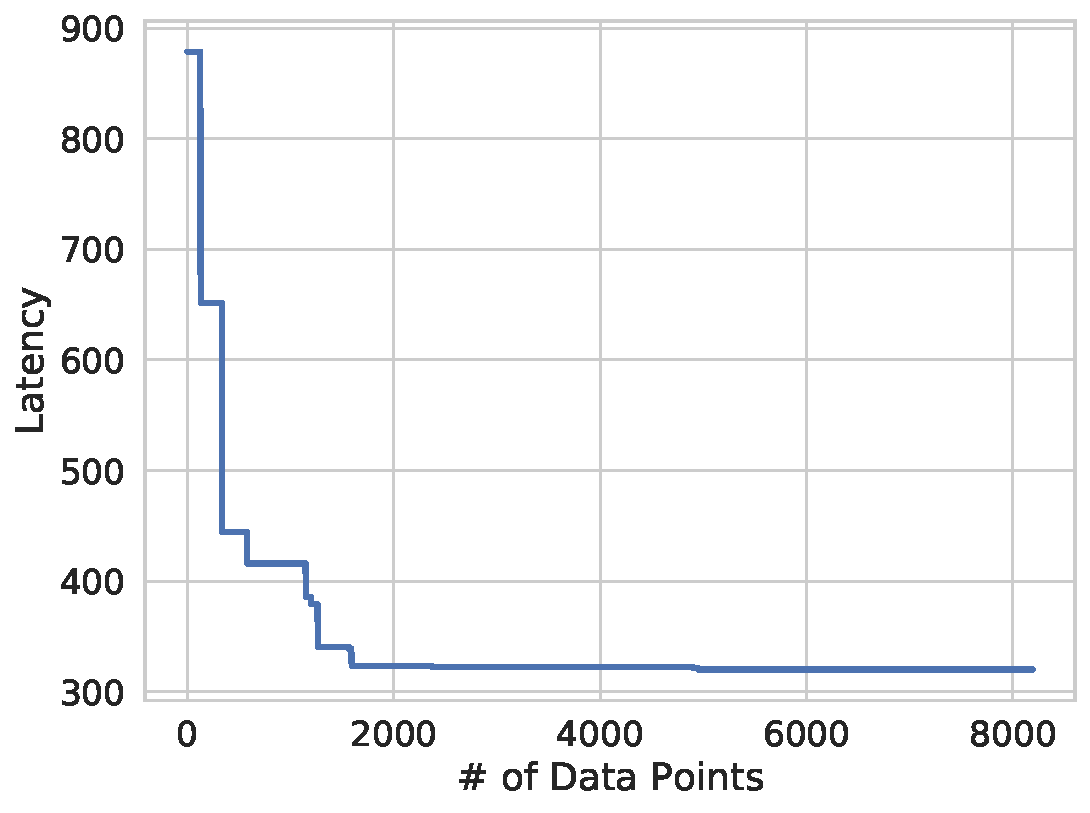
\includegraphics[width=0.32\linewidth]{chapters/prime/figs/convergence/mobilenetedge.pdf}}
\subfloat[MobileNetV2]{\label{fig:conv_v2}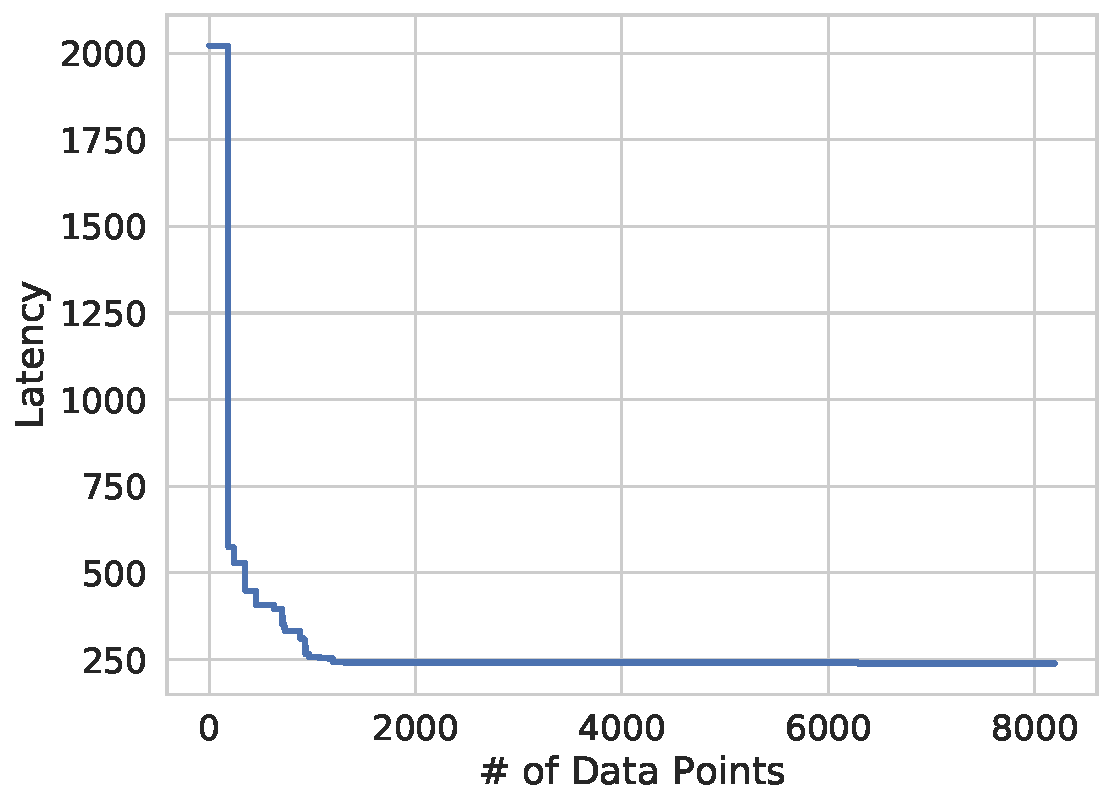
\includegraphics[width=0.32\linewidth]{chapters/prime/figs/convergence/mobilenetv2.pdf}}
\subfloat[MobileNetV3]{\label{fig:conv_v3}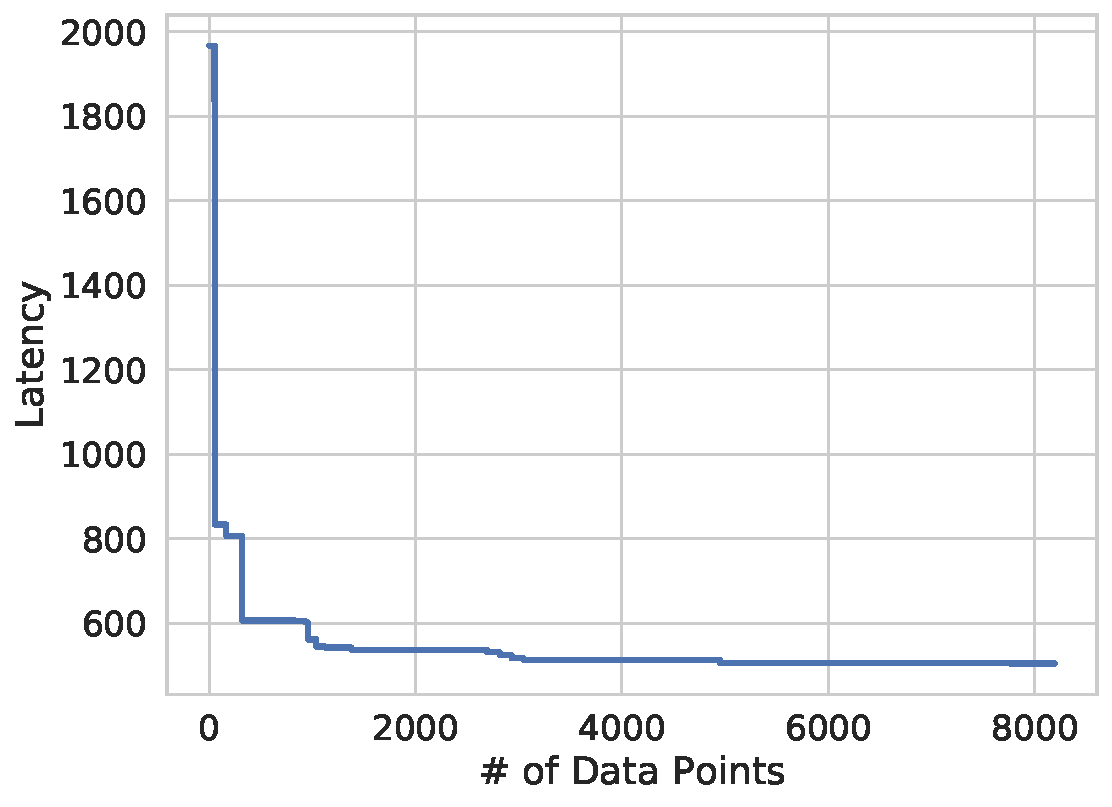
\includegraphics[width=0.32\linewidth]{chapters/prime/figs/convergence/mobilenetv3.pdf}}\\
%
\subfloat[\mfour]{\label{fig:conv_m4}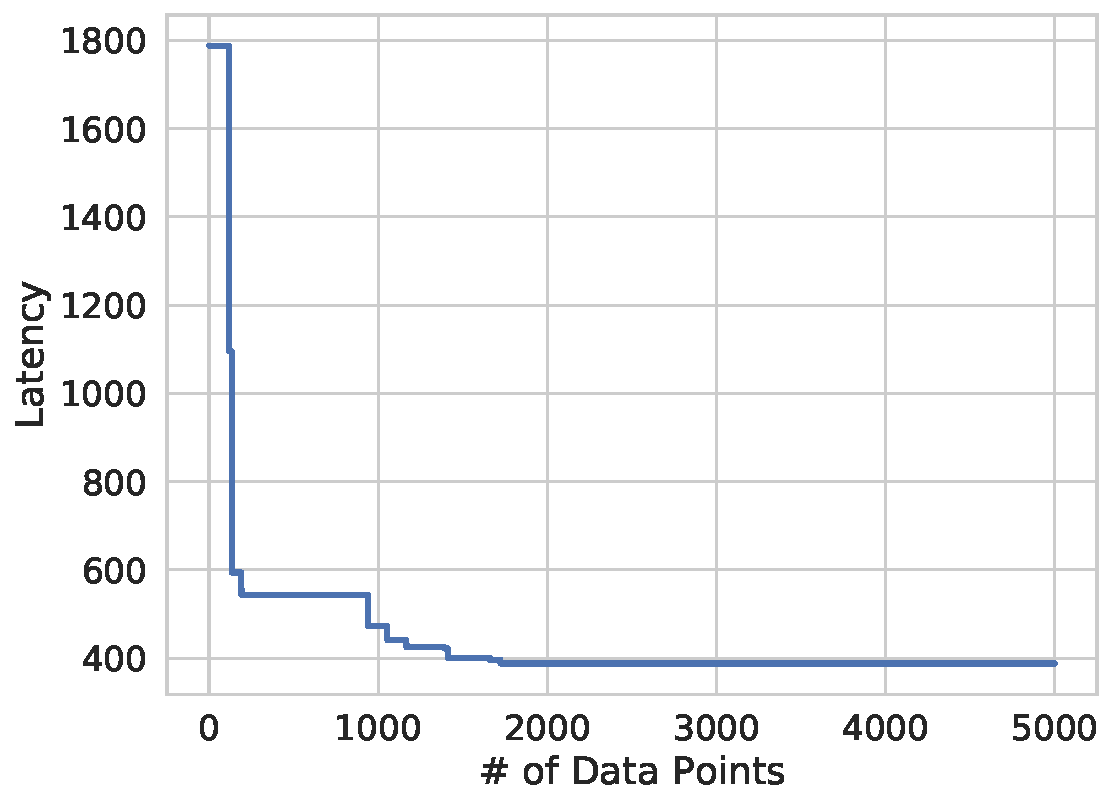
\includegraphics[width=0.32\linewidth]{chapters/prime/figs/convergence/m4.pdf}}
\subfloat[\mfive]{\label{fig:conv_m5}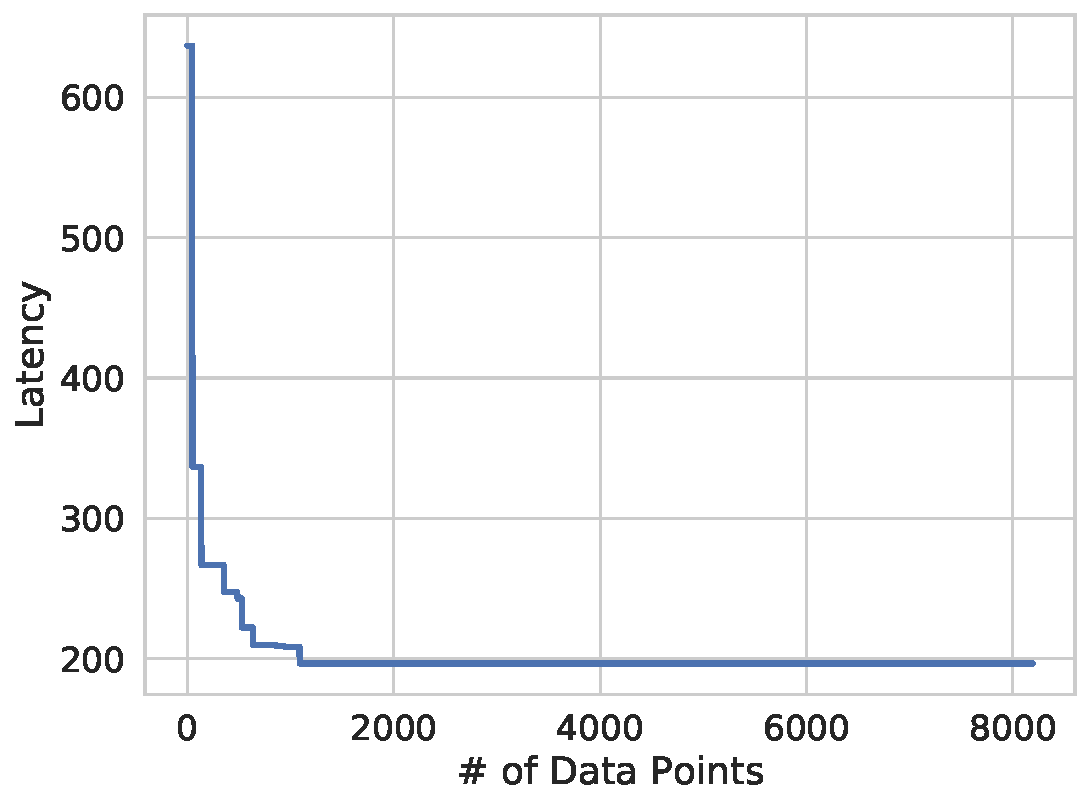
\includegraphics[width=0.32\linewidth]{chapters/prime/figs/convergence/m5.pdf}}
\subfloat[\msix]{\label{fig:conv_m6}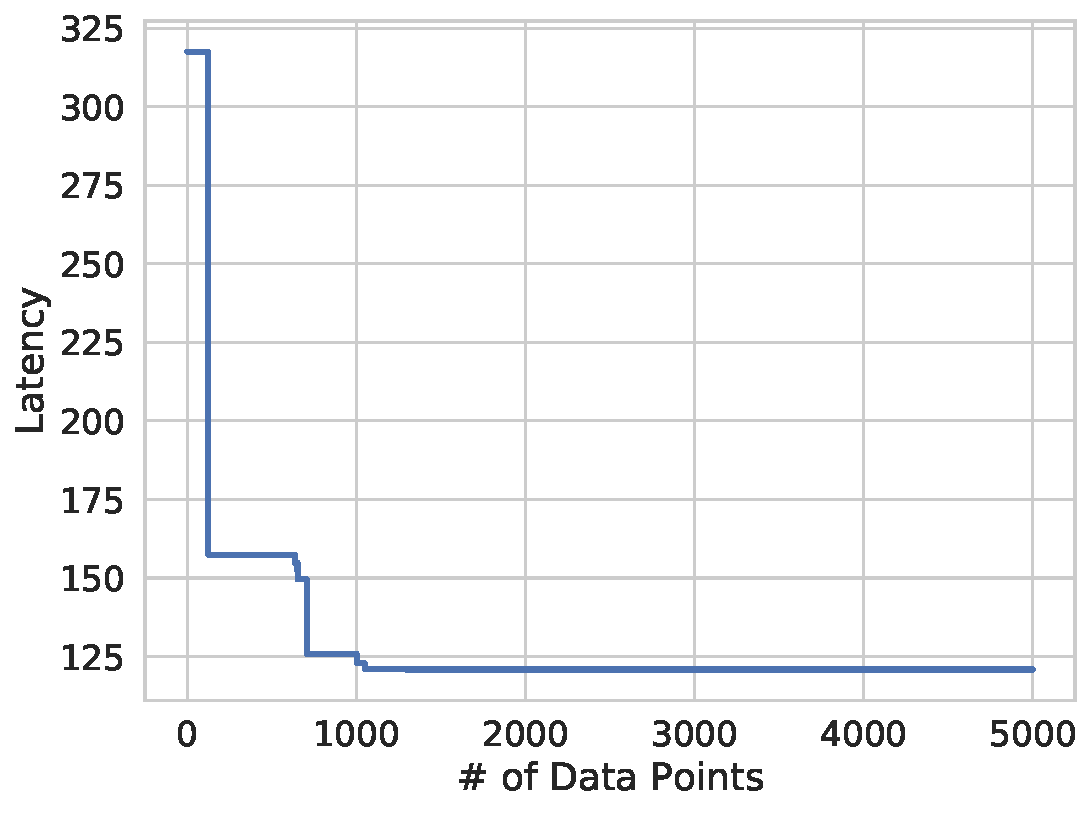
\includegraphics[width=0.32\linewidth]{chapters/prime/figs/convergence/m6.pdf}}\\
%
\subfloat[U-Net]{\label{fig:conv_unet}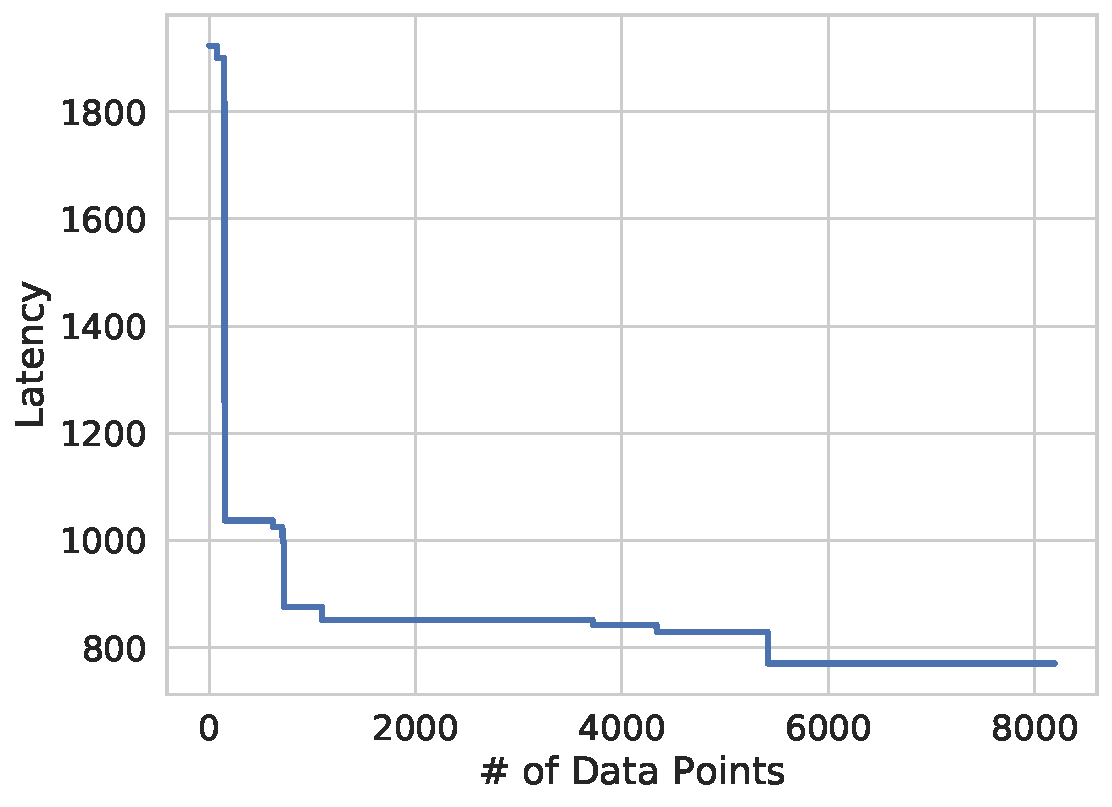
\includegraphics[width=0.32\linewidth]{chapters/prime/figs/convergence/unet.pdf}}
\subfloat[t-RNN Dec]{\label{fig:conv_rnn_dec}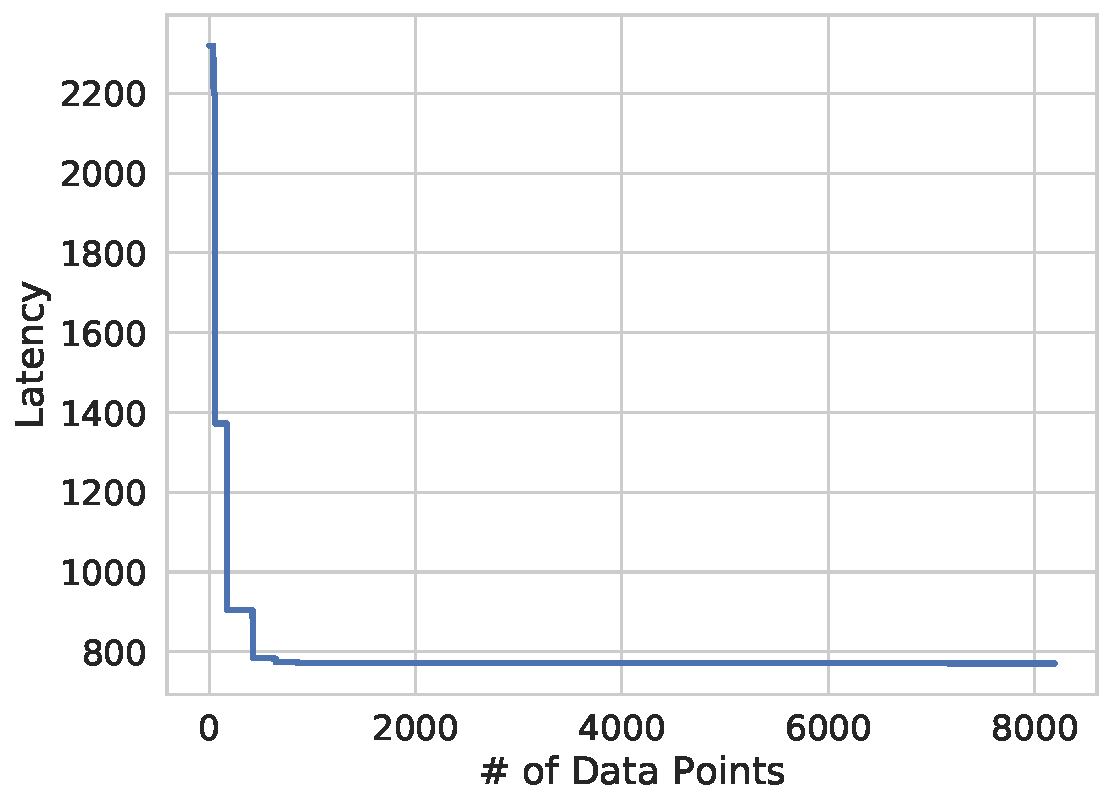
\includegraphics[width=0.32\linewidth]{chapters/prime/figs/convergence/rnn-dec.pdf}}
\subfloat[t-RNN Enc]{\label{fig:conv_enc}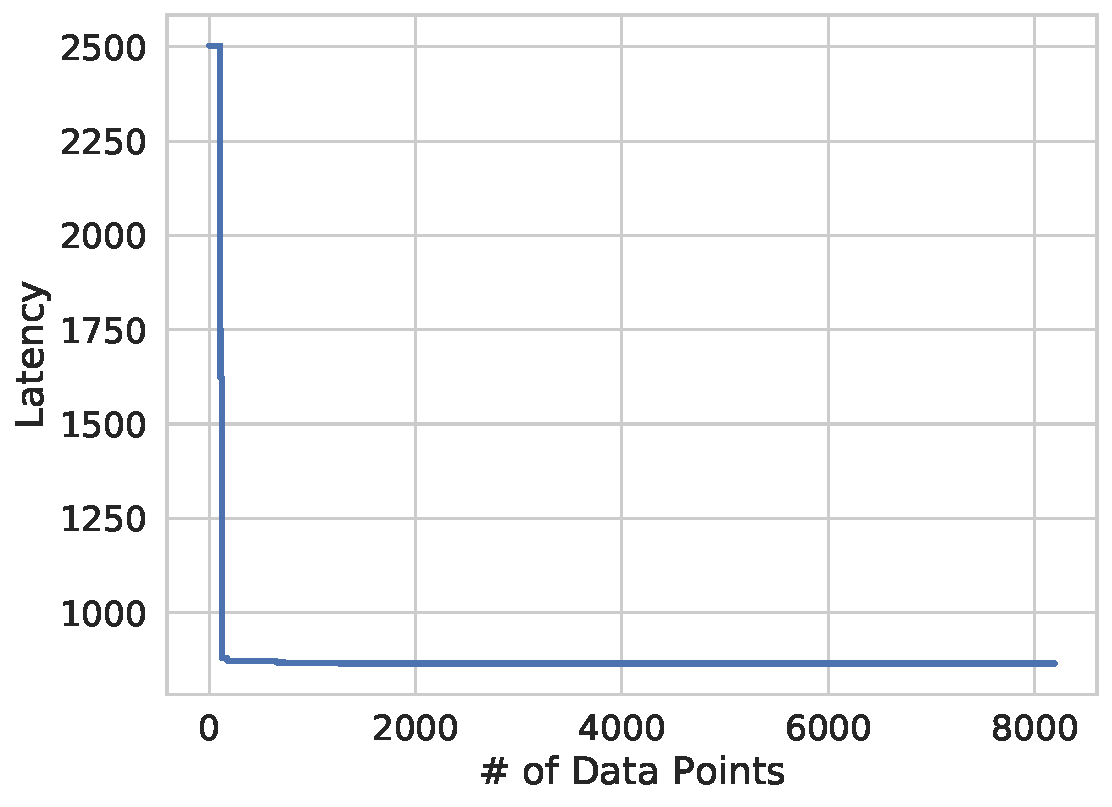
\includegraphics[width=0.32\linewidth]{chapters/prime/figs/convergence/rnn-enc.pdf}}
\caption{\review{Optimization behavior of Firefly optimizer (Online Evolutionary). Observe that the optimization procedure converges and plateaus very quickly (at least 1000 iterations in advance) and hence we stop at 8000 iterations. In the case of t-RNN Enc and t-RNN Dec, we find that the evolutionary algorithm performs poorly and we suspect this is because it saturates quite quickly to a suboptimal solution and is unable to escape. This is also evident from Figures~\ref{fig:conv_rnn_dec} and \ref{fig:conv_enc}, where we observe that online optimization plateaus the fastest for these RNN applications. }}
\label{fig:convergence_curves} 
% \vspace{-0.5cm}
\end{figure}


\subsubsection{{Exact Hyperparameters Found By Our Cross-Validation Strategy}}

{In this section, we present the exact hyperparameters found by our cross-validation strategy discussed in Section~\ref{sec:method}. To recap, our offline cross-validation strategy finds the early stopping checkpoint and selects the values of $\alpha$ and $\beta$ in Equation~\ref{eqn:final_training} that attain the highest rank correlation on a held-out validation set consisting of top 20\% of the dataset feasible samples. The values of $\alpha$, $\beta$ and checkpoint selected for the experiments in Table 3, Table 4, Table 5 and 6 are shown in Table~\ref{table:hparams}.} 


\begin{table*}[t!]
\small
\centering
\renewcommand{\arraystretch}{1.1}
\vspace*{-0.05cm}
\caption{\label{table:hparams} \footnotesize \review{Hyperparameters $\alpha$, $\beta$ and checkpoint index (measured in terms of gradient steps on the learned conservative model) for \primemethodname\ found by our \textbf{offline} cross-validation strategy discussed in Section~\ref{sec:method}, that is based on the Kendall's rank correlation on the validation set (note that no simulator queries were used to tune hyperparameters). In the case of the multi-task and zero-shot scenarios, when training on more than one application, the batch size used for training \primemethodname\ increases to $N$-fold, where $N$ is the number of applications in the training set, therefore we likely find that even a few gradient steps are good enough.}}
\vspace{-0.1cm}
\resizebox{1.0\textwidth}{!}{\begin{tabular}{l|l|l|l|l}
\toprule
\textbf{Table}&\textbf{Application}&\textbf{$\alpha$}&\textbf{$\beta$}&\textbf{Checkpoint Index}\\\midrule
Table~\ref{table:results_single_task} & MobileNetEdgeTPU & 0.01 & 5.0 & 80000 \\\hline
Table~\ref{table:results_single_task} & MobileNetV2 & 5.0 & 5.0 & 120000 \\\hline
Table~\ref{table:results_single_task} & MobileNetV3 & 5.0 & 0.01 & 80000 \\\hline
Table~\ref{table:results_single_task} & \mfour & 0.1 & 0.0 & 80000 \\\hline
Table~\ref{table:results_single_task} & \mfive & 5.0 & 1.0 & 80000 \\\hline
Table~\ref{table:results_single_task} & \msix & 1.0 & 1.0 & 60000 \\\hline
Table~\ref{table:results_single_task} & U-Net & 0.0 & 1.0 & 100000 \\\hline
Table~\ref{table:results_single_task} & t-RNN Dec & 1.0 & 0.0 & 60000 \\\hline
Table~\ref{table:results_single_task} & t-RNN Enc & 0.0 & 0.1 & 60000 \\\midrule \hline
Table~\ref{table:results_multi_task} & MobileNet (EdgeTPU, V2, V3) & 5.0 & 0.01  & 60000 \\\hline
Table~\ref{table:results_multi_task} & MobileNet (V2, V3), \mfive, \msix & 0.0 & 5.0 & 30000 \\\hline
Table~\ref{table:results_multi_task} & MobileNet (EdgeTPU, V2, V3), \mfour, \mfive, \msix & 0.5 & 0.0 & 100000 \\\hline
Table~\ref{table:results_multi_task} & MobileNet (EdgeTPU, V2, V3), \mfour, \mfive, \msix, t-RNN Enc (Area 29.0) & 0.0 & 1.0  & 20000 \\\hline
Table~\ref{table:results_multi_task} & MobileNet (EdgeTPU, V2, V3), \mfour, \mfive, \msix, t-RNN Enc (Area 100.0) & 0.0 & 0.0 & 20000 \\\hline
Table~\ref{table:results_multi_task} & MobileNet (EdgeTPU, V2, V3), \mfour, \mfive, \msix, U-Net, t-RNN (Enc, Dec) (Area 29.0) &  0.01 & 0.01 & 10000 \\\hline
Table~\ref{table:results_multi_task} & MobileNet (EdgeTPU, V2, V3), \mfour, \mfive, \msix, U-Net, t-RNN (Enc, Dec) (Area 100.0) & 0.01 & 0.1  & 20000  \\\midrule\hline
Table~\ref{table:zero_shot} & Train (Zero-Shot): MobileNet (EdgeTPU, V3) & 5.0 & 0.01 & 60000\\\hline
Table~\ref{table:zero_shot} & Train (Zero-Shot): MobileNet (V2, V3), \mfive, \msix &  0.0 & 5.0 & 30000  \\\hline
Table~\ref{table:zero_shot} & Train (Zero-Shot): MobileNet (EdgeTPU, V2, V3), \mfour, \mfive, \msix, t-RNN Enc (Area 29.0) & 0.0 & 1.0 & 20000 \\\hline
Table~\ref{table:zero_shot} & Train (Zero-Shot): MobileNet (EdgeTPU, V2, V3), \mfour, \mfive, \msix, t-RNN Enc (Area 100.0) & 0.1 & 5.0 & 20000 \\ \midrule\hline
Table~\ref{table:dla_shi} & MobileNetV2 (NVDLA) & 0.0 & 1.0 & 40000 \\\hline
Table~\ref{table:dla_shi} & MobileNetV2 (ShinDianNao) & 0.0 & 0.0 & 40000 \\\hline
Table~\ref{table:dla_shi} & ResNet 50 (NVDLA) & 0.01 & 0.0 & 40000 \\\hline
Table~\ref{table:dla_shi} & ResNet 50 (ShinDianNao) & 0.0 & 0.0 & 75000 \\\hline
Table~\ref{table:dla_shi} & Transformer (NVDLA) & 0.01 & 1.0 & 200000 \\\hline
Table~\ref{table:dla_shi} & Transformer (ShinDianNao) & 0.0 & 0.1 & 100000 \\
\bottomrule
% \CC \textbf{Geomean of \primemethodname's Improvement}&\CC---&\CC~\texttt{\textbf{1.0$\times$}}&\CC~\texttt{\textbf{1.06$\times$}}&\CC~\texttt{\textbf{3.75$\times$}}\\
% \bottomrule
\end{tabular}}
\vspace{-0.1cm}
\end{table*}

%
\subsection{Details of Architecting Accelerators for Multiple Applications Simultaneously}
%
\label{sec:appx_multi_task_tsne}
Now we will provide details of the tasks from Table~\ref{table:results_multi_task} where the goal is to architect an accelerator which is jointly optimized for multiple application models.
%
For such tasks, we augment data-points for each model with the context vector $c_k$ from Table~\ref{tab:models} that summarizes certain parameters for each application.
%
For entries in this context vector that have extremely high magnitudes (e.g., model parameters and number of compute operations), we normalize the values by the sum of values across the applications considered to only encode the relative scale, and not the absolute value which is not required.
%
To better visualize the number of feasible accelerators for joint optimization, Figure~\ref{fig:tsne_overlap} show the tSNE plot (raw architecture configurations are used as input) of high-performing accelerator configurations. The blue-colored dots are the jointly feasible accelerators in the combined dataset, and note that these data points are no more than 20-30 in total. The highlighted red star presents the best design suggested by \primemethodname\ with average latency of 334.70 (Table~\ref{table:results_multi_task}).
%
This indicates that this contextual, multi-application problem poses a challenge for data-driven methods: these methods need to produce optimized designs even though very few accelerators are jointly feasible in the combined dataset.
% 
Despite this limitation, \primemethodname\ successfully finds more efficient accelerator configurations that attain low latency values on each of the applications jointly, as shown in Table~\ref{table:results_multi_task}.

\begin{figure}[t]
    \centering
    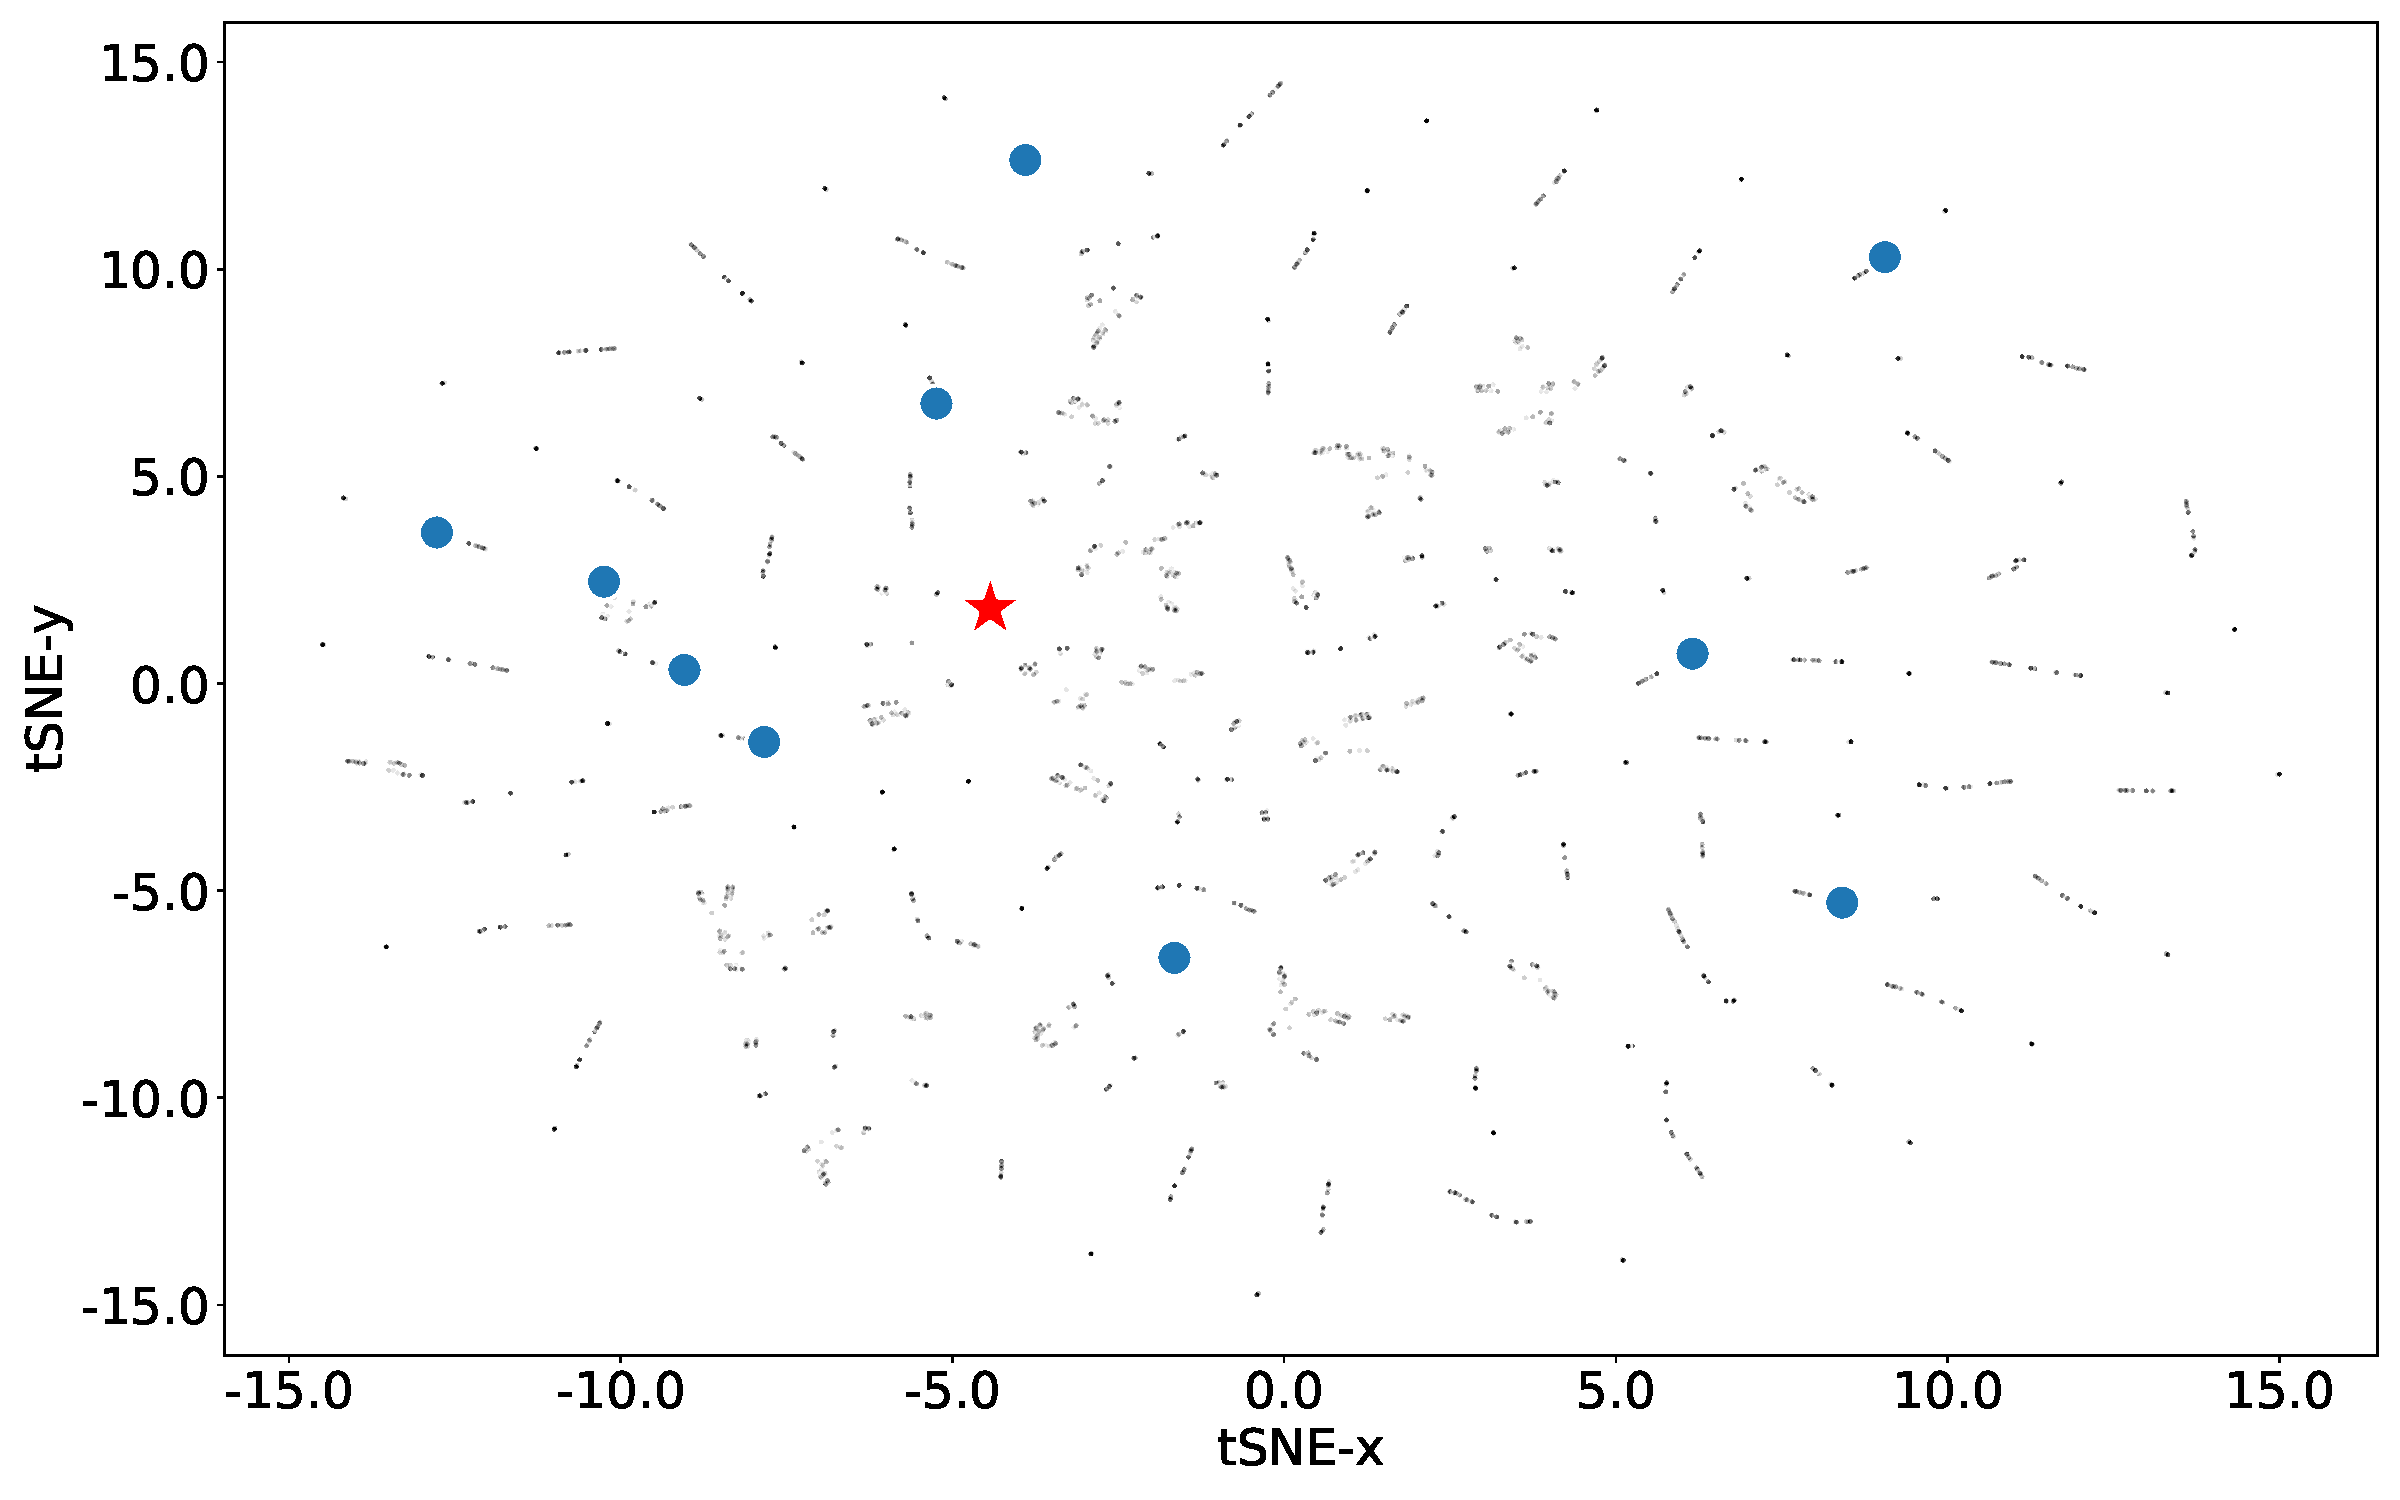
\includegraphics[width=0.7\textwidth]{chapters/prime/figs/tsne/tsne-overlap.pdf}
    \caption{tSNE plot of the joint dataset and randomly sampled infeasible data points. The blue points show the accelerator configurations that are jointly feasible for all the applications. The highlighted point with red star shows the best design proposed by \primemethodname\. The rest of the points show the infeasible points.}
    \label{fig:tsne_overlap}
    \vspace{-0.1in}
\end{figure}
%


\subsection{Dataset Sensitivity to Accelerator Parameters}
\label{sec:app_ds_sensitivity}
%
We visualize the sensitivity of the objective function (e.g. latency) with respect to the changes in certain accelerator parameters, such as memory size (Table~\ref{tab:arch_params}), in Figure~\ref{fig:appx_ds_memory}, illustrating this sensitivity.
%
As shown in the Figure, the latency objective that we seek to optimize can exhibit high sensitivity to small variations in the architecture parameters, making the optimization landscape particularly ill-behaved.
%
Thus, a small change in one of the discrete parameters, can induce a large change in the optimization objective.
%
This characteristic of the dataset further makes the optimization task challenging. 


\section{Overview of Accelerators and Search Space}
\label{sec:dla_shi_fast}
%
This section briefly discuss the additional accelerators (similar to \citep{kao2020confuciux}) that we evaluate in this work, namely NVDLA~\citep{nvidia} and ShiDianNao~\citep{shidiannao}, and their corresponding search spaces.

\niparagraph{NVDLA: Nvidia Deep Learning Accelerator}
%
NVDLA~\citep{nvdla} is an open architecture inference accelerator designed and maintained by Nvidia.
%
In compared to other inference accelerators, NVDLA is a weight stationary accelerator. That is, it retains the model parameters on each processing elements and parallelizes the computations across input and output channels.
%
NVDLA-style dataflow accelerators generally yield better performance for the computations of layers at the later processing stages. This is because these layers generally have larger model parameters that could benefit from less data movement associated to the model parameters.

\niparagraph{ShiDianNao: Vision Accelerator}
%
Figure~\ref{fig:shi_dla} shows the high-level schematic of ShiDianNao accelerator~\citep{shidiannao}.
%
ShiDianNao-style dataflow accelerator is an output-stationary accelerator.
%
\begin{figure}[t!]
\centering
    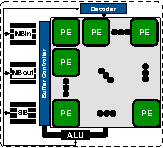
\includegraphics[width=0.35\linewidth]{chapters/prime/figs/accelerator/shidian.pdf}
    \caption{Overview of ShiDianNao dataflow accelerator. This dataflow accelerators exhibits an output-stationary dataflow where it keeps the partial results stationary within each processing elements (PEs).}
    \label{fig:shi_dla}
    \vspace{-0.1in} 
\end{figure}
That is, it keeps the partial results inside each PE and instead move the model parameters and input channel data. 
%
As such, in compared to NVDLA-style accelerators, ShiDianNao provides better performance for the computations of the layers with large output channels (generally first few layers of a model).

\niparagraph{Search space of dataflow accelerators.}
%
We follow a similar methodology as \citep{kao2020confuciux} to evaluate additional hardware accelerators, discussed in the previous paragraphs.
%
We use MAESTRO~\citep{maestro}, an analytical cost model, that supports the performance modeling of various dataflow accelerators.
%
In this joint accelerator design and dataflow optimization problem, the total number of parameters to be optimized is up to 106---the tuple of (\# of PEs, Buffers) per per model layer---with each parameter taking one of 12 discrete values. This makes the hardware search space consist of $\approx$~2.5$\times10^{114}$ accelerator configurations.
%
We also note that while the method proposed in~\citep{kao2020confuciux} treats the accelerator design problem as a sequential decision making problem, and uses reinforcement learning techniques, \primemethodname\ simply designs the whole accelerator in a single step, treating it as a model-based optimization problem.

\begin{figure}[t]
    \centering
    %
    \subfloat[]{
    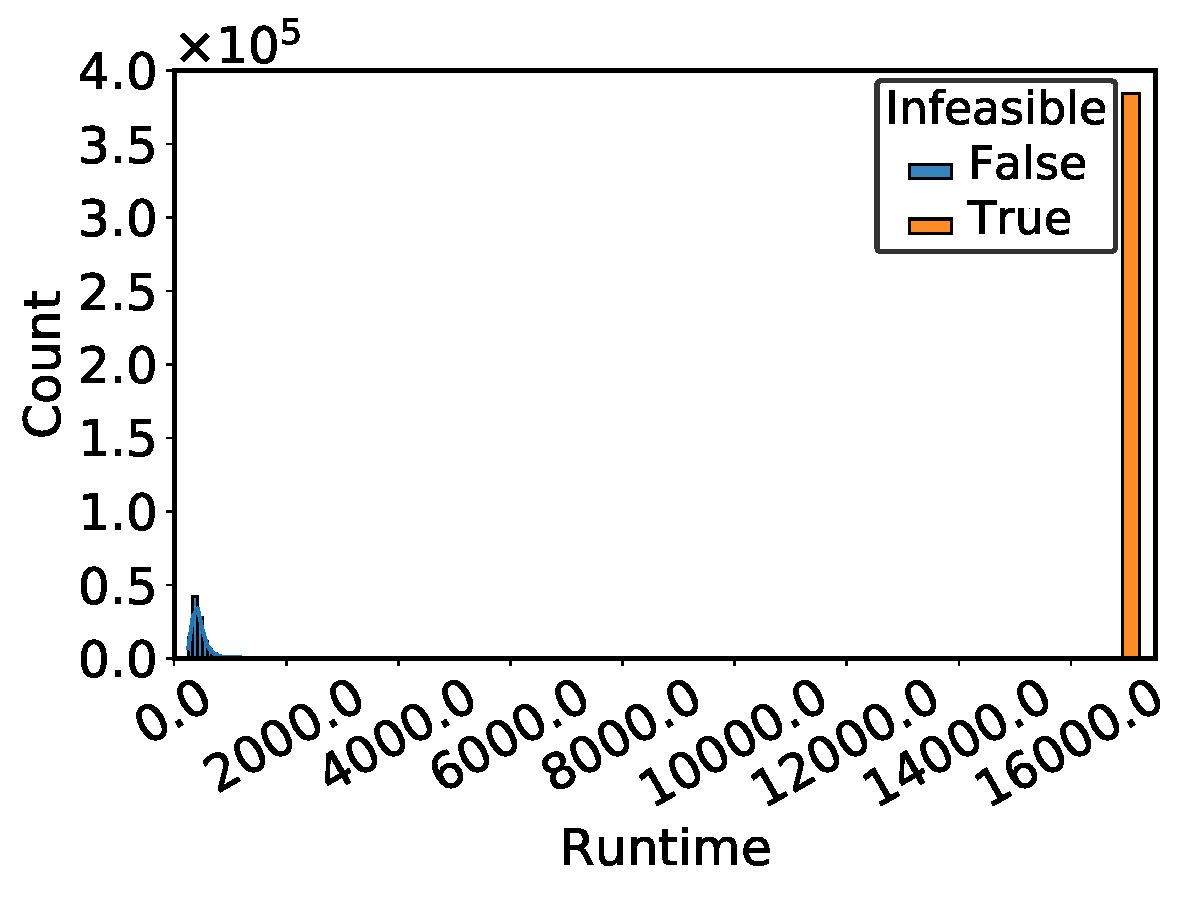
\includegraphics[width=0.45\textwidth]{chapters/prime/figs/dataset/dist.pdf}
    \label{fig:appx_ds_dist}}
    %
    \subfloat[]{
    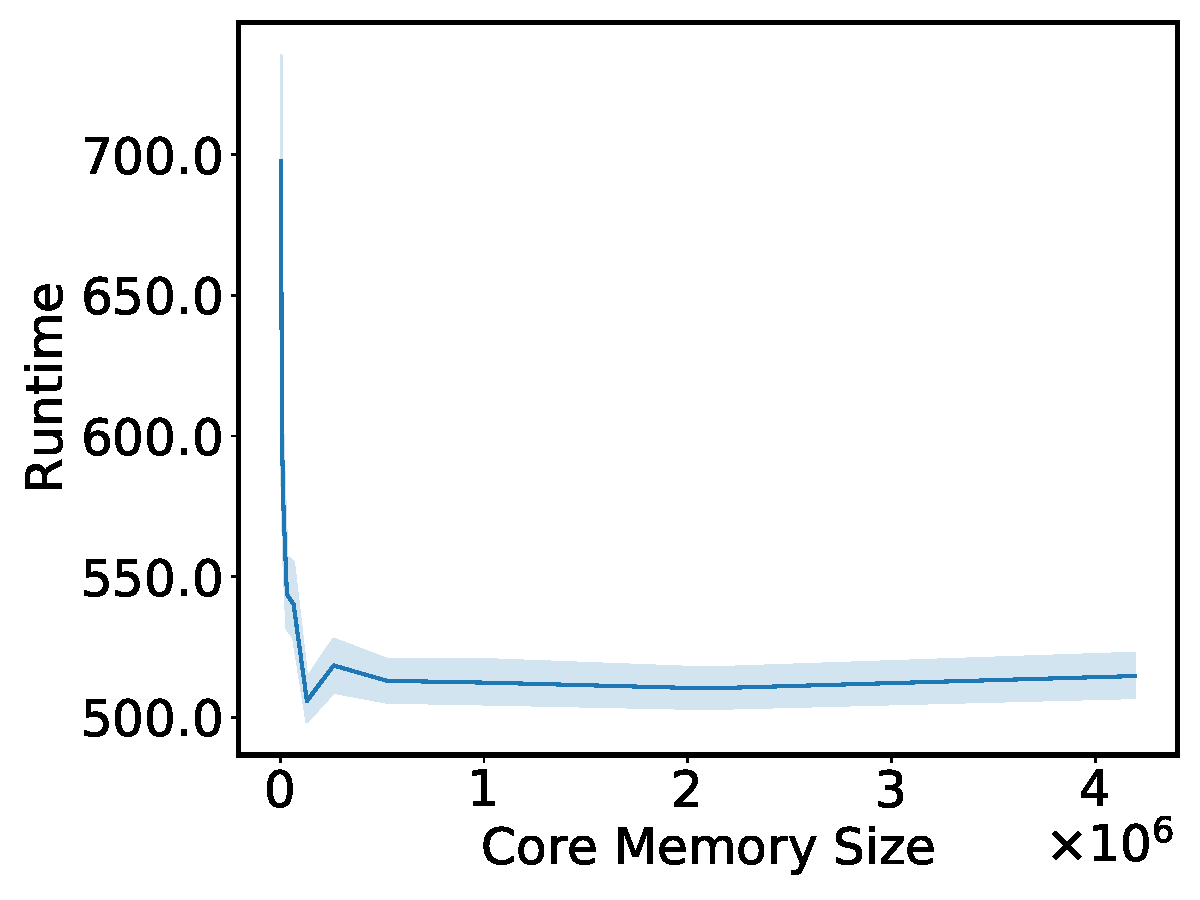
\includegraphics[width=0.45\textwidth]{chapters/prime/figs/dataset/core-memory.pdf}
    \label{fig:appx_ds_memory}}
    \caption{The (a) histogram of infeasible (orange bar with large score values)/feasible (blue bars) data points and (b) the sensitivity of runtime to the size of core memory for the MobileNetEdgeTPU~\citep{efficientnet:2020} dataset.} 
    \label{fig:appx_ds}
    \vspace{-0.4cm}
\end{figure}

\begin{table*}[t!]
\small{
\begin{center}
% \vspace*{0.1cm}
\caption{\footnotesize {The evaluated applications, their model parameter size, number of compute operations, and normalized compute-to-memory ratio.}}
\label{tab:compute_memory_ratio}
\vspace{-0.1in}
\resizebox{0.8\textwidth}{!}{\begin{tabular}{l|c|r|r}
\toprule
\textbf{Name}&\textbf{Model Param}&\textbf{\# of Compute Ops.}&\textbf{Normalized Compute-to-Memory Ratio}\\\midrule
{\textbf{MobileNetEdgeTPU}}&3.87~MB&1,989,811,168&1.38e-1\\\hline
{\textbf{MobileNetV2}}&3.31~MB&609,353,376&4.96e-2\\\hline
{\textbf{MobileNetV3}}&5.20~MB&449,219,600&2.33e-2\\\hline
\textbf{\mfour}&6.23~MB&3,471,920,128&1.5e-1\\\hline
\textbf{\mfive}&2.16~MB&939,752,960&1.17e-1\\\hline
\textbf{\msix}&0.41~MB&228,146,848&1.5e-1\\\hline
\textbf{U-Net}&3.69~MB&13,707,214,848&1.0\\\hline
\textbf{t-RNN Dec}&19~MB&40,116,224&\textbf{5.68e-4}\\\hline
\textbf{t-RNN Enc}&21.62~MB&45,621,248&\textbf{5.68e-4}\\
\bottomrule
\end{tabular}}
\end{center}
\vspace{-0.1cm}
}
% \vspace{-0.6cm}
\end{table*}

\begin{figure}[ht]
    \centering
    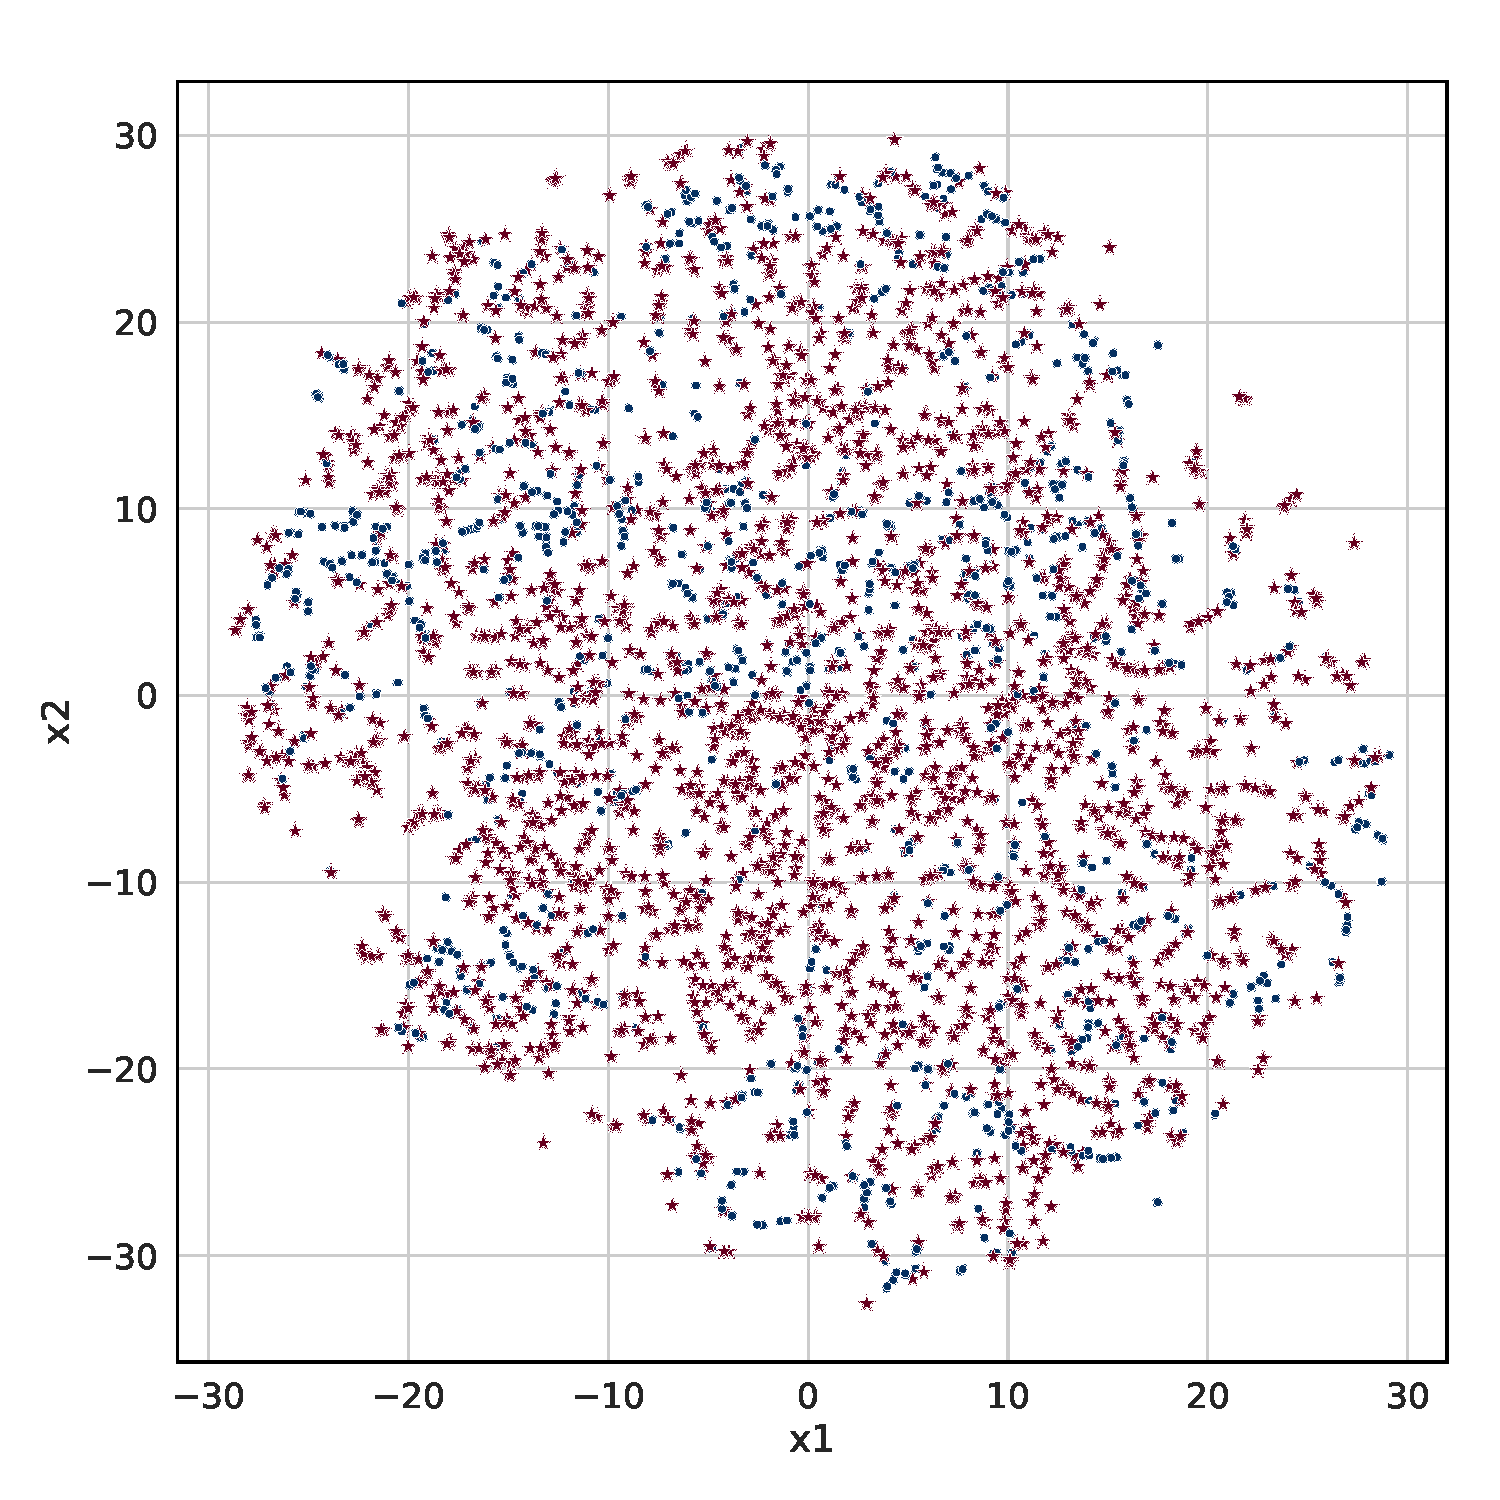
\includegraphics[width=0.45\textwidth]{chapters/prime/figs/tsne/tsne_infeasible.pdf}
    \caption{tSNE plot of the infeasible and feasible hardware accelerator designs. Note that feasible designs (shown in blue) are embedded in a sea of infeasible designs (shown in red), which makes this a challenging domain for optimization methods.}
    \label{fig:tsne_infeasible}
    \vspace{-0.1in}
\end{figure}

\begin{figure}[ht]
    \centering
    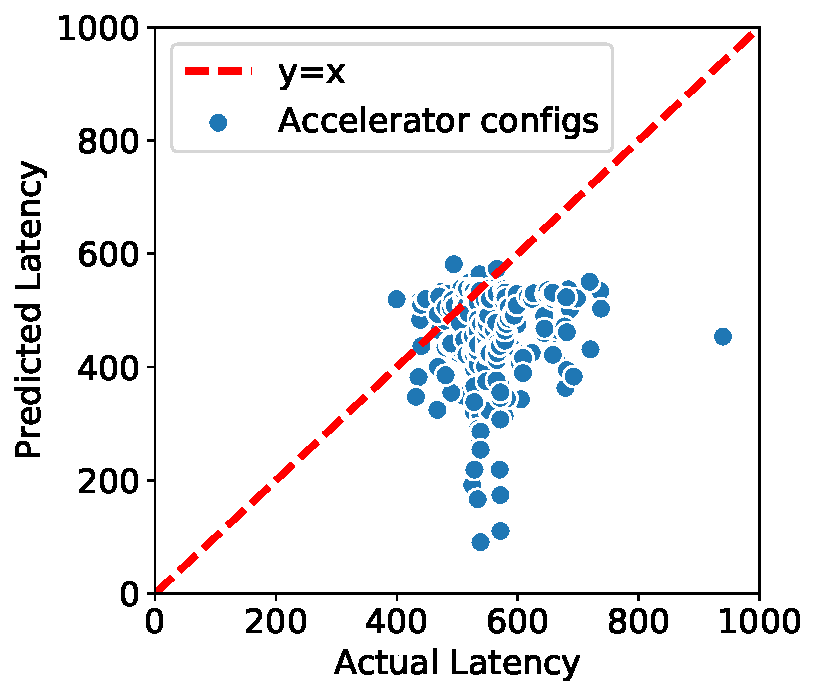
\includegraphics[width=0.4\textwidth]{chapters/prime/figs/results/overestimation.pdf}
    \caption{To verify if the overestimation hypothesis--that optimizing an accelerator against a na\"ive standard surrogate model is likely to find optimizers that appear promising under the learned model, but do not actually attain low-latency values--in our domain, we plot a calibration plot of the top accelerator designs found by optimizing a na\"ively trained standard surrogate model. In the scatter plot, we represent each accelerator as a point with its x-coordinate equal to the actual latency obtained by running this accelerator design in the simulator and the y-coordinate equal to the predicted latency under the learned surrogate. Note that for a large chunk of designs, the predicted latency is much smaller than their actual latency (i.e., these designs lie beneath the $y=x$ line in the plot above). This means that optimizing designs under a na\"ive surrogate model is prone to finding designs that appear overly promising (i.e., attain lower predicted latency values), but are not actually promising. This confirms the presence of the overestimation hypothesis on our problem domain.}
    \label{fig:cali_plot}
    \vspace{-0.1in}
\end{figure}

\begin{figure}[ht]
    \centering
    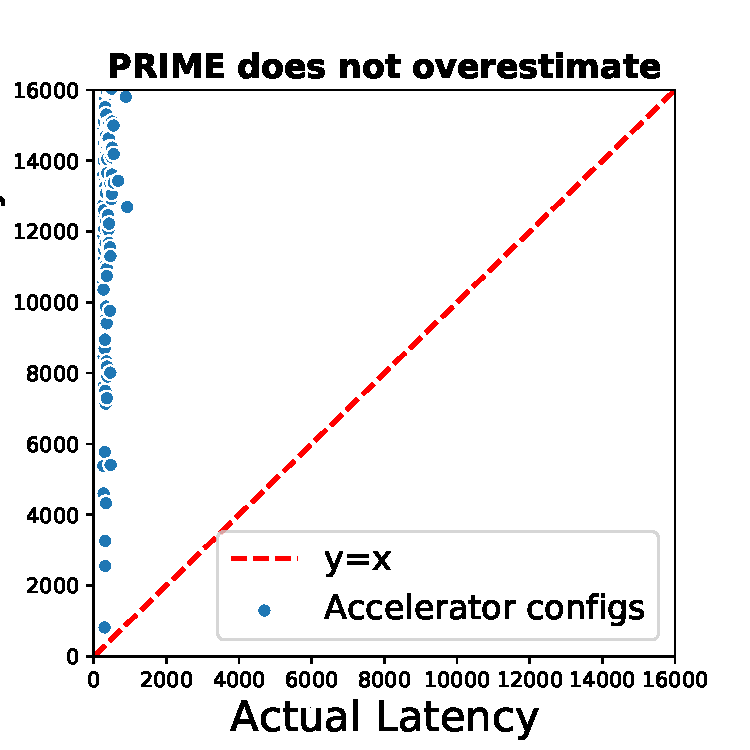
\includegraphics[width=0.4\textwidth]{chapters/prime/figs/overestimation_prime.pdf}
    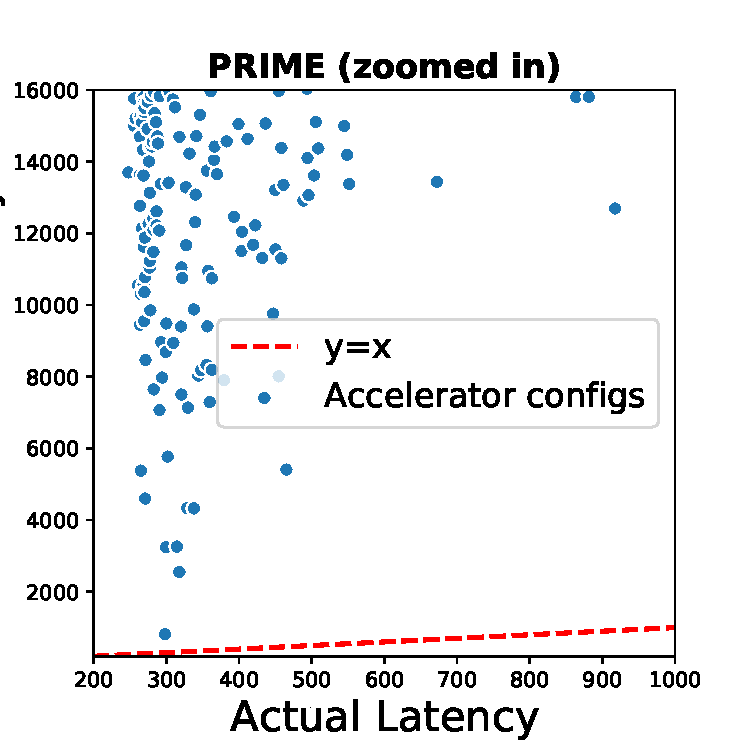
\includegraphics[width=0.4\textwidth]{chapters/prime/figs/zoomed_in.pdf}
    \caption{\review{Plot showing the calibration plot of the predicted (y-axis) and actual latencies (x-axis) of accelerators found by \primemethodname. Compared to Figure~\ref{fig:cali_plot}, observe that all the acclerator configurations lie above $y=x$, meaning that \primemethodname\ predicts a higher latency (y-axis) compared to the actual latency. This means that \primemethodname\ does not think that accelerators that attain high-latency values under the simulator, are actually good.  We also provide a zoomed-in version of the plot on the right, which shows that there are accelerators do have meaningfully distinct latency predictions under \primemethodname. Observe in the zoomed-in plot that the designs that attain small predicted latencies also perform relatively better under the actual latency compared to the designs that attain larger predicted latency of $\sim$ 14000-16000 under the \primemethodname\ surrogate. Optimizing against \primemethodname\ is still effective because optimization just needs relative correctness of values, not absolutely correct latency predictions.}}
    \label{fig:overestimation_prime_plot}
    \vspace{-0.1in}
\end{figure}

% \newpage

\section{{Subset of Applications for Good Zero-Shot Performance}}
%
\begin{table*}[t]
\small
\centering
\vspace*{0.0cm}
\caption{\label{table:zero_shot_all_2} \footnotesize \review{Additional ablation study under zero-shot setting when the test applications include all the nine evaluated models (e.g. MobileNet (EdgeTPU, V2, V3), \mfour, \mfive, \msix, t-RNN Dec, t-RNN Enc, U-Net). Lower latency is better. From \textbf{left} to \textbf{right}: the applications used to train the surrogate model in \primemethodname, the area constraint of the accelerator, \primemethodname's (best, median) latency.}}
\vspace{-0.1cm}
\resizebox{0.9\textwidth}{!}{% <------ Don't forget this %
\begin{tabular}{l|l|l}
\toprule
\textbf{Train Applications}&\textbf{Area}&\textbf{\primemethodname} \textbf{(best, median)} \\\midrule
% Area 29
\textbf{(1)} MobileNet~(V2, V3), \mfive, \msix&29~mm$^2$&({426.65}, {427.35})\\\hline
% Area 29
\textbf{(2)} MobileNet~(V2, V3), \mfive, t-RNN Enc&29~mm$^2$&({461.79}, {464.87})\\\hline
% Area 29
\textbf{(3)} MobileNet~(EdgeTPU, V2, V3), \mfour, \mfive, \msix, t-RNN Enc&29~mm$^2$&({426.65}, {427.94})\\\bottomrule
\end{tabular}% <------ Don't forget this %
}
% \vspace{-0.2cm}
\end{table*}
%
{In this section, we present the results of an ablation study with the goal to identify a subset of applications such that training on data from only these applications yields good zero-shot performance across all the nine applications studied in this work.
%
Since we cannot train \primemethodname\ for every subset of applications because the space of subsets of all applications is exponentially large, we utilized some heuristics in devising the subset of applications we would train on, with the goal to make interesting observations that allow us to devise rough guidelines for performing application selection.}

{\textbf{Our heuristic for devising subsets of applications:} Building on the intuition that applications with very different compute to memory ratios (shown in Table~\ref{tab:compute_memory_ratio}) may require different accelerator designs -- for example, if our goal is to run a compute-intensive application, we likely need an accelerator design with more compute units -- we study two subsets of training applications: \textbf{(1)} MobileNetV2, MobileNetV3, \msix, \mfive, and \textbf{(2)} MobileNetV2, MobilenetV3, \mfive, t-RNN Enc.
%
Note that, these two combinations only differ in whether some RNN application was used in training or not.
%
As shown in Table~\ref{tab:compute_memory_ratio}, the t-RNN applications admit a very different compute to memory ratio, for instance, while this ratio is $5.68e-4$ for t-RNN Enc and t-RNN Dec, it is much different $\sim 0.01-0.2$ for other models MobileNetEdgeTPU, MobileNetV2, MobileNetV3, \mfive, and \msix. This means that likely t-RNN Enc and Dec will require different kinds of accelerators for good performance compared to the other applications.}

{\textbf{Results:} We present the performance of zero-shot evaluating the designed accelerator obtained by training on combinations \textbf{(1)} and \textbf{(2)}, and also the accelerator obtained by training on \textbf{(3)} seven applications from Table~\ref{table:zero_shot} in Table~\ref{table:zero_shot_all_2} as reference. We make some key takeaways from the results: 
}
\begin{itemize}
    \item The performance of both configuration \textbf{(1)} and training with seven applications (\textbf{(3)}, last row of Table~\ref{table:zero_shot_all_2}) are similar.
    \item In case \textbf{(2)}, when the training applications consist of four applications in which one application is t-RNN Enc, with drastically different compute to memory ratio (Table~\ref{tab:compute_memory_ratio}), the performance on an average across all applications becomes slightly worse (compare the performance in \textbf{(2)} vs \textbf{(3)}).
\end{itemize}

{\textbf{Conclusion and guidance on selecting good applications:} The above results indicate that only a few applications (e.g., four applications in case \textbf{(1)}) can be enough for good performance on all nine applications. While this set may not be not minimal, it is certainly a much smaller set compared to the nine applications considered.
Adding an RNN application in case \textbf{(2)} increases latency in compared to case \textbf{(1)}, because t-RNN Enc likely admits a very different optimal accelerator compared to the other applications due to a very different compute/memory ratio, which in turn skews the generalization of the surrogate learned by \primemethodname\ when trained only on this limited set of four applications. However, when seven applications are provided in case \textbf{(3)}, even when the set of training applications includes t-RNN, its contribution on the \primemethodname\ surrogate is reduced since many other compute intensive applications are also provided in the training set and the resulting accelerator performs well.}
%

{\textbf{Practitioner guidance:} The primary practitioner guidance we can conclude here is that \emph{the models used for training must be representative of the overall distribution of the target models that we want to zero-shot generalize to}. Since a number of our applications are compute intensive, we were able to simply utilize set \textbf{(1)} to attain good performance on all the applications. On the other hand, in case \textbf{(2)}, when the t-RNN Enc application was over-represented -- while seven of nine applications we considered were primarily compute intensive, one out of four applications we used for training in case \textbf{(2)} were memory intensive -- this hurt performance on the overall set.
%
Therefore, we believe that ensuring that the training subset of applications is adequately aligned with the overall set of applications in terms of compute/memory ratio statistic is imperative for favorable zero-shot performance.}

{\textbf{For a practitioner deciding between zero-shot generalization and additional data collection}, it may make sense to test if the target application admits a similar value of the compute to memory ratio as an already existing application. If it does, then the practitioner might be able to utilize the zero-shot generalization, as is indicated with the good performance of case \textbf{(1)}, whereas if the compute/memory ratio is heavily different from any seen application, zero-shot generalization to the target application may be worse. Finally, making sure that the training applications adequately reflect the compute/memory ratio statistic for the overall target set is important.}
